%
% You may wish to use some of the following options of the iitthesis
% package:
%
% fullpageDraft      avoid the margins necessary for proper binding and
%   just view or print a draft.
% beforeDefense      make the personal acknowledgements invisible;
%   use this to print the copies you submit initially to the grad school
%   for sending to the opponent panel, i.e. thesis readers (who shouldn't
%   see those parts). For the final submission, after having successfully
%   defended - drop this option.
% noabbrevs          avoid generation of a notation & abbreviations list
%
% Additionally, you must specify the degree for which you're writing
% your thesis (MSc/PhD/MArch etc.)
%
\documentclass[MSc, beforeDefense]{misc/iitthesis}


% Definitions of info fields for the thesis - subject, advisor,
% faculty, acknowledgements, etc. etc. The thesis-fields file 
% contains Hebrew text, and should use the UTF-8 character set
% encoding (not iso-8859-8-i or windows codepage 1255).
% This file contains definitions of various fields used
% in various places throughout the thesis (in the title
% pages mostly). Whatever isn't define here has some
% default (and usually irrelevant) text.

\authorEnglish{Antonio Abu Nassar}
\authorHebrew{אנטוניו אבו נסאר}

\titleEnglish{Semantic Symmetry in Transducers}
\titleHebrew{סימטריה סמנטית במשרנים}

\disciplineEnglish{Computer Science}
\disciplineHebrew{מדעי המחשב}

\supervisionEnglish{This research was carried out under the supervision of Dr.~Shaull Almagor, in the Faculty of Computer Science.}
\supervisionHebrew{המחקר בוצע בהנחייתו של ד"ר שאול אלמגור, בפקולטה למדעי המחשב.}

\GregorianDateEnglish{June 2022}
\GregorianDateHebrew{יוני \textenglish{2022}}
\JewishDateEnglish{Sivan 5782}
\JewishDateHebrew{סיון התשפ"ב}

%\financialAcknowledgementEnglish{The Technion's funding of this research is hereby acknowledged.}
%\financialAcknowledgementHebrew{הכרת תודה מסורה לטכניון על מימון מחקר זה.}

\publicationInfoEnglish{%
Some results in this thesis have been published as articles by the author and research collaborators in conferences and journals during the course of the author's masters research period, the most up-to-date versions of which being:

\butcheredbibliography{front/pubinfo.bib}
}

\publicationInfoHebrew{%
חלק מן התוצאות בחיבור זה פורסמו כמאמרים מאת המחבר ושותפיו למחקר בכנסים ובכתבי-עת במהלך תקופת מחקר המגיסטר של המחבר, אשר גרסאותיהם העדכניות ביותר הינן:%

\begin{otherlanguage}{english}%
\butcheredbibliography{front/pubinfo.bib}
\end{otherlanguage}%
}

\addbibresource{back/general.bib}
% \thesisbibstyle{trad-alpha}


% Personal acknowledgements (are only used for the post-exam
% version)
\personalAcknowledgementEnglish{
\newfontfamily\Calligraphic[Ligatures=TeX]{Miama Nueva}
\newfontfamily\SpecialHebrew{Stam Ashkenaz CLM}

First and foremost, I would like to thank my advisor, Dr. Shaull Almagor, for being an incredible supervisor and research leader, a fun partner and friend, and for being consistently supportive.

I would also like to express my appreciation for the committee members for making my defense an enjoyable moment, and the kind donors of my fellowship at the Technion and the PBC scholarship program for guaranteeing me a quiet mind and a calm spirit determined on excellence.

Thank you loads, my friends and family who supported me all the way, especially~my dear parents, Naief and Angela, for the warm love and support and for receiving me back home during the Covid times with loving open arms. Thanks for having my back!

%[Thank you especially Teta, Nonna and Nonno, Gabi, Yuhanna, George, Raafat, Firas and Perla, Rabea, Mikhail, Noor, Juna, Dunia and the rest of my buddies who encouraged me the most along the way.]

Sincere gratitude goes also to the team I worked with at IBM during the summer, who showed great interest in my thesis and gave me the opportunity to present it at~work. %, especially to Shai Doron who gave me the opportunity to present it at work.

An endless, cordial thank you to my other family, {\Calligraphic UCO Galilee}, for being a shelter and a stronghold, for the prayers and all the blessings I received by their intercessions.

Finally, thank You {\Calligraphic God} for the gift of life and for giving humanity a chance to learn a glimpse or two about Your eternal Wisdom and Beauty.

}

\personalAcknowledgementHebrew{

ראשית, ברצוני להודות למנחה שלי, ד״ר שאול אלמגור, על היותו מנחה ומנהיג מחקר מדהים, שותף כיפי וחבר, ועל תמיכתו הנמשכת.

ברצוני להביע את הערכתי גם לחברי הוועדה שהפכו את ההגנה לרגע מהנה, לתורמים האדיבים של מלגתי בטכניון ולתכנית המלגות של ות״ת על שהבטיחו לי ראש שקט ורוח רגועה הנחושה למצוינות.

תודה רבה לכם, חבריי ובני משפחתי שתמכו בי לאורך כל הדרך, במיוחד הוריי היקרים, נאיף~ואנג'לה, על האהבה החמה והתמיכה ועל שקיבלתם אותי חזרה הביתה בתקופת הקורונה בזרועות פתוחות ואוהבות. תודה שיש לי אתכם!

תודה כנה מגיעה גם כן לצוות שאיתו עבדתי בחברת יב״מ במהלך הקיץ, שגילה עניין רב בתזה שלי ונתן לי את ההזדמנות להציג אותה בעבודה.

תודה אינסופית מכל הלב למשפחתי השנייה, 
\textenglish{\Calligraphic UCO Galilee},
על היותה מחסה ומצודה, על התפילות וכל הברכות שקיבלתי דרכה.

לבסוף, תודה לך
{\SpecialHebrew אלוהים}
על מתנת החיים ועל שנתת לאנושות הזדמנות ללמוד הצצה או שתיים על חוכמתך ויופייך הנצחיים.

}


% A separate file for the abstract - in English and in Hebrew, so
% you must make sure it's also in the UTF-8 character set encoding.
%
% This file contains the abstract part of your thesis - in English and
% in Hebrew (within \abstractEnglish and \abstractHebrew respectively).
%
% Notes:
% - This file uses the UTF-8 character set encoding for the Hebrew
%   text not to get garbled. Keep it that way.
% - Assuming your thesis is mainly in English, Graduate School 
%   regulations mandate the following lengths for the abstracts:
%
%      Language    Min. Length   Max. Length
%     ---------------------------------------
%      English       200 words     500 words
%      Hebrew        500 words   2,000 words
%
%   so that the Hebrew abstract typically has some content from
%   the English introduction and an overview of the results, not
%   present in the English; it is not just a translation.

\abstractEnglish{
% For a nicer bullet in itemize
\renewcommand\textbullet{\textcolor{BrickRed}{\ensuremath{\bigstar}}}

Model checking is a verification paradigm for systems, where we are given a system and a specification and we check whether every possible computation of the system satisfies the specification.

Often, systems over multiple processes exhibit some type of symmetry in their structure or their behaviour. Symmetry is also commonly manifested in the specifications of multiple process systems.
When such symmetries are present in the system or the specification, they can be exploited by the designer and the verification algorithm to alleviate some of the complexity of model checking, as well as to gain insight into the behaviour of the system. For instance, symmetric systems enable the designer to use only representative specifications where iteration over the process identities was formerly needed.
Thus, we want to decide whether a given system or specification exhibits symmetry.

Symmetry is not a well-defined concept and might come in various forms, each capturing a different characteristic behaviour. In this work, we focus on \emph{process symmetry}, where every process $j$ has a corresponding input and output signal $i_j$ and $o_j$, and the input and output alphabets of the model are $\tI$ and $\tO$ respectively.
Process symmetry addresses the scenario where the identities of the processes may be scrambled -- that is, permuted.
For example, if the input $\{i_1,i_2\}$ is generated, the system might actually receive an input $\{i_7,i_4\}$.
Then, a system exhibits process symmetry if, intuitively, its outputs are permuted in a similar way to the inputs.
Unfortunately, deterministic systems that are process symmetric are extremely naive, as process symmetry is too restrictive for them.

In our setting, each of the system and the specification are modelled by a finite-state machine called a \emph{transducer}. In addition, words are partitioned into rounds, and a transducer $\cT$ is \emph{$k$-round symmetric} if for every permutation $\pi$ of the signals and for every input word $x$, we can scramble the letters within each round in $\pi(x)$ to obtain $x'$, such that the output of $\cT$ on $x'$ is itself a scramble of the output of $\cT$ on $x$. In other words, when $\cT$ is round symmetric, there is a way to scramble the permuted input, so that the resulting output is a scramble of the permuted output (i.e. the ``expected'' output in process symmetry).

Round symmetry is \emph{semantic}: it does not consider the structure, rather the behaviour of the system. Round symmetry gives rise to the following decision problems:
\begin{itemize}
	\item In \emph{fixed round symmetry} we are given a transducer $\cT$ and $k>0$, and we need to decide whether $\cT$ is $k$-round symmetric.
	\item In \emph{existential round symmetry} we are given a transducer $\cT$, and we need to decide whether there exists $k>0$ such that $\cT$ is $k$-round symmetric.
\end{itemize}

Notice that round symmetry defines a property of a transducer. The way we approach the decision problems is by first translating the definition of symmetry to a definition of a relation between two transducers, called \emph{round simulation}, then showing that round symmetry can be reduced to round simulation, we solve it as such.

A transducer $\cT_2$ \emph{$k$-round simulates} transducer $\cT_1$ if for every input word $x$, we can scramble the letters within each round in $x$, such that the output of $\cT_2$ on the scrambled word is itself a scramble of the output of $\cT_1$ on $x$.
In fact, we consider a somewhat more elaborate setting, by also allowing the inputs to $\cT_1$ to be restricted to some regular language $\fL$.

The mapping between the input words for $\cT_1$ and the scrambled input for $\cT_2$ is called the \emph{simulation mapping} and is also studied in the continuation of this work.

Round symmetry and round simulation -- the decision problems and their solutions, upper and lower bounds and the simulation mapping -- are the main contribution of this work.
Additionally, several more notions of symmetry are presented and discussed, including variations of round symmetry, and symmetry in the setting of infinite words.

We use tools and techniques from logic, algebra and automata theory.
} % end of English abstract

\abstractHebrew{
בדיקת מודלים היא פרדיגמת אימות למערכות, בה אנו פועלים להכרעה האם מערכת עומדת במפרט נתון.
% לעתים קרובות, מערכת מפגינה סוג כלשהו של סימטריה במבנה שלה או בהתנהגות שלה. סימטריות כאלה יכולות להיות מנוצלות על ידי מעצב התוכנה כדי להקל חלק מהמורכבות של בדיקת מודלים, כמו גם כדי לקבל תובנה לגבי התנהגות המערכת. לפיכך, אנו מעוניינים להחליט אם מערכת נתונה מפגינה סימטריה.
לעתים קרובות, מערכות מרובות תהליכים מפגינות סוג כלשהו של סימטריה במבנה שלהן או בהתנהגות שלהן. סימטריה מתבטאת בדרך כלל גם במפרטים אשר מערכות מרובות תהליכים נבדקות נגדם.
כאשר קיימת סימטריה במערכת או במפרט, היא יכולה להיות מנוצלת על ידי המעצב ואלגוריתם האימות כדי להקל חלק מהמורכבות של בדיקת מודלים, כמו גם כדי לקבל תובנה לגבי התנהגות המערכת. לדוגמה, מערכות סימטריות מאפשרות למעצב להשתמש רק במפרטים מייצגים שבהם היה צורך בעבר באיטרציה על זהויות התהליכים.
לפיכך, אנו מעוניינים להחליט אם מערכת נתונה מפגינה סימטריה.

סימטריה אינה מושג מוגדר היטב ועשויה לבוא בצורות שונות, שכל אחת מהן תופסת התנהגות אופיינית אחרת.
בעבודה זו, אנו מתמקדים
ב\emph{סימטריית תהליכים},
בה לכל תהליך
$j$
יש אות קלט ופלט מתאימים
$i_j$ ו- $o_j$,
ואלפבית הקלט והפלט של המודל הם
$\tI$ ו- $\tO$
בהתאמה.
סימטריית תהליכים מתייחסת לתרחיש שבו זהויות התהליכים עשויות להיות מעורבבות 
\textenglish{--}
כלומר, עברו התמרה.
לדוגמה, אם הקלט
$\{i_1,i_2\}$
נוצר, המערכת עשויה לקבל למעשה קלט
$\{i_7,i_4\}$.
לאחר מכן, מערכת מפגינה סימטריית תהליכים אם, באופן אינטואיטיבי, הפלטים שלה עוברים התמרה בצורה דומה לקלטים.
לרוע המזל, מערכות דטרמיניסטיות שמפגינות סימטריית תהליכים הן תמימות ביותר, שכן סימטריית תהליכים מגבילה מדי עבורן.

% אנו מציגים מושג של סימטריה סמנטית במודל החישובי הנקרא משרן
% (\textenglish{transducer}),
% ומדגימים את ההגדרות וההתנהגויות שהוא לוכד, כמו גם מציגים את הבעיות האלגוריתמיות הרלוונטיות ואת הפתרונות שלהן.
% בפרט, אנו מציגים את הרעיון של 
% \emph{סימולציה בסיבובים}, 
% שתועלתו היא בכך שניתן ליישם אותה בתחום הסימטריה של תהליכים, למשל במערכות תזמון
% (\textenglish{schedulers}).

בהגדרה שלנו, המערכת ואף המפרט ממודלים על ידי מכונת מצבים סופית הנקראת
\emph{משרן}.
בנוסף,
% בסימטריה שאנו מגדירים, סימטריה בסיבובים, 
מילת הקלט של המשרן מחולקת לתתי מילים זרות באורך קבוע שנקראות סיבובים, ונאמר שמשרן
$\cT$
הינו
\emph{סימטרי בסיבובים של 
$k$}
אם עבור כל תמורה של אותות
$\pi$,
וכל מילת קלט 
$x$,
נוכל לערבב את האותיות בכל סיבוב בקלט לאחר ההתמרה,
$\pi(x)$,
כדי לקבל $x'$,
כך שהפלט של
$\cT$
על
$x'$
הוא עצמו ערבוב של תוצאת התמורה על הפלט של
$\cT$
על
$x$.
במילים אחרות, כאשר
$\cT$
הוא סימטרי בסיבובים, יש דרך לערבב את הקלט המתומר, כך שהפלט המתקבל הוא ערבוב של הפלט המתומר
(שהוא הפלט ”הצפוי“ בסימטריית תהליכים).

סימטריה בסיבובים היא
\emph{סמנטית}
בכך שהיא לא מתחשבת במבנה, אלא בהתנהגות המערכת.
סימטריה בסיבובים מובילה לבעיות ההכרעה הבאות:
\begin{itemize}
\item
בבעיה 
\emph{הקבועה}
של סימטריה בסיבובים, 
ניתן לנו משרן
$\cT$ וקבוע $k>0$,
ועלינו להחליט אם
$\cT$ 
הוא סימטרי בסיבובים של
$k$.
\item
בבעיה 
\emph{הקיומית}
של סימטריה בסיבובים, 
ניתן לנו משרן
$\cT$,
ועלינו להחליט אם קיים
$k>0$
כך ש-
$\cT$
הוא סימטרי בסיבובים של
$k$.
\end{itemize}

שימו לב שסימטריה בסיבובים מגדירה תכונה של משרן.
הדרך בה אנו ניגשים לבעיות ההחלטה היא על ידי תרגום ההגדרה של סימטריה להגדרה של קשר בין שני משרנים, הנקרא
\emph{סימולציה בסיבובים},
ואז, לאחר שנראה כי ניתן לצמצם סימטריה בסיבובים לסימולציה בסיבובים, אנו פותרים אותה ככזו.

משרן
$\cT_2$
\emph{מסמלץ}
משרן
$\cT_1$
\emph{בסיבובים של
$k$}
אם עבור כל מילת קלט
$x$, 
נוכל לערבב את האותיות בכל סיבוב ב-
$x$,
כך שהפלט של
$\cT_2$
על המילה לאחר הערבוב היא עצמה ערבוב של הפלט של
$\cT_1$
על
$x$.
% לבסוף, שני משרנים נקראים
% \emph{שקולים בסיבובים של 
% $k$}
% אם הם מסמלצים זה את זה.
למעשה, אנו נותנים הגדרה קצת יותר משוכללת, בכך שאנו מאפשרים גם לקלט ל-
$\cT_1$
להיות מוגבל לשפה רגולרית נתונה
$\fL$.

בהתאם, בעיות ההכרעה הנוצרות מההגדרה של סימולציה בסיבובים הן האם 
$\cT_2$
מסמלץ את
$\cT_1$
בסיבובים של
$k$,
(1) כאשר
$k$
ניתן כקלט, ו-(2) עבור
$k$
בכמת קיומי (קרי, עבור
$k$
כלשהו).
% אנו גם מספקים חסמים תחתונים לבעיות (חלקם עם פערים שנותרו), 
% ולאחר מכן אנו מראים שניתן לצמצם את בעיית הסימטריה בסיבובים לסימולציה בסיבובים ולפתור אותה ככזו.

המיפוי בין מילות הקלט עבור
$\cT_1$
לבין הקלט המעורבב עבור
$\cT_2$
נקרא
\emph{מיפוי הסימולציה}
והוא נדון בהמשך עבודה זו.

סימטריה בסיבובים וסימולציה בסיבובים 
\textenglish{--}
בעיות ההחלטה ופתרונותיהן, הגבול העליון והתחתון ומיפוי הסימולציה
\textenglish{--}
הם התרומה העיקרית של עבודה זו.
בנוסף, מוצגים ונדונים עוד כמה מושגים של סימטריה, כולל וריאציות של סימטריה עגולה וסימטריה בהגדרה של אינסוף מילים.

\subsection*{\texthebrew{תקציר לפתרון של בעיות ההכרעה}}

נגדיר תחילה את המודל העיקרי שאיתו אנו עובדים.
\emph{משרן}
(\textenglish{transducer})
הינו מכונת מצבים הדומה לאוטומט סופי דטרמיניסטי, פרט לכך שלכל מצב מוצמדת אות פלט, וריצה של משרן על מילת קלט
$w$
מחזירה פלט באותו אורך, לפי המצבים שהמילה
$w$
עברה בהם. בניגוד לאוטומטים, אין משמעות לקבלה של מילים במשרן.

כאמור, אנו פותרים את בעיות ההכרעה של סימולציה בסיבובים, ומכאן גם נקבל פתרון עבור בעיית הסימטריה בסיבובים.

הבעיה הראשונה היא המקרה הקל מבין שניהם. אנו מתחילים לפתור אותה בהגדרת כלי שהוא אוטומט סופי אי-דטרמיניסטי שאנו מכנים סגור-תמורות 
(\textenglish{Permutation Closure}).

אוטומט סגור-תמורות מתקבל מהמשרן
$\cT$
ואורך הסיבוב 
$k$. 
בו, כל רצף של
$k$
מעברים במשרן המקורי נותן מעבר יחיד באוטומט החדש. יתר על כן, זהו מעבר שאינו מודע לסדר האותיות. זה נותן שהאוטומט למעשה עונה על התכונה שלפיה בחרנו את שמו: סגירות תחת תמורות, משמע שכל התמורות של אותו זוג מילות קלט ופלט מתנהגות באופן זהה זו לזו.

כדי לבנות אוטומט זה, השתמשנו באוטומט ביניים דטרמיניסטי בשם
\textenglish{Trace}
שבעצם מוציא את אותיות הפלט מהמצבים לקשתות הנכנסות.

בהישען על כלי זה, אנו מגיעים ללמה האומרת כי עבור משרנים נתונים
$\cT_1$, $\cT_2$
ואורך סיבוב
$k$,
סימולציה בסיבובים מתקיימת בין
$\cT_1$
ו-
$\cT_2$
אם ורק אם יש הכלה בין השפות של אוטומטי סגור-תמורות של
$\cT_1$
ושל
$\cT_2$.

אכן, אינטואיטיבית, אם נקבל איזשהו קלט עבור
$\cT_1$
והפלט המתאים לו, ההכלה הזו אומרת שיש תמורה כלשהי של הקלט כך שהפלט הוא עצמו גם תמורה של הפלט הנתון.

מכיוון שצמצמנו את הבעיה לבעיית ההכלה של אוטומטים אי-דטרמיניסטיים, תוצאה ישירה היא שהבעיה היא במחלקת הסיבוכיות
$\PSPACE$.
 למעשה, אנו גם מראים שהבעיה הינה
$\PSPACE$-שלמה.

כעת, במקרה הקיומי, אנו שואלים אם יש איזה אורך סיבוב שעבורו מתקיימת סימולציה סיבובית. אנו עושים זאת על ידי מציאת חסם עליון לאורך הסיבוב המינימלי שעבורו מתקיימת סימולציה סיבובית. זה נותן לנו חסם עליון סופי לקבוצת האורכים שאנו צריכים לבדוק מולם, מה שהופך את הבעיה לניתנת להכרעה.

גם כאן אנו משתמשים בכלים. הראשון הוא הטיפוס של אותיות באוטומטים. טיפוס של אות נותן תיאור של האופן שבו מצב המכונה משתנה כאשר אות זו נקראת. בהתחשב בסוגי האותיות באוטומט סגור-תמורות, אנו עוברים לדבר על קבוצת כל הטיפוסים שנצפו באוטומט, שאנו מכנים ב- ״פרופיל הטיפוס״ של האוטומט.

אנו מעוניינים בפרופילי הטיפוס של אוטומטי סגור-תמורות עבור אורכי סיבוב הולכים וגדלים. ישנו מספר סופי של אפשרויות לפרופילי טיפוס, עד כדי ריבוי. עוד אנו טוענים שיש אורך סיבוב כלשהו, שלאחריו לא מופיעים פרופילי טיפוס חדשים. כלומר, בהגעתנו אליו, כבר נראה את כל פרופילי הטיפוס שאנו הולכים לראות. זה לוקח אותנו לכלי הבא: אנו מוכיחים את המשפט הזה על ידי תרגום שלו לבעיה 
\emph{בחשבון פרסבורגר}, 
ופותרים אותו הודות למחקר בלוגיקה.

אורך סיבוב זה נותן לנו בעצם את המטרה שלנו, על ידי התבוננות בתוצאה הסופית הזו: אם פרופילי הטיפוס שווים לאורכי סיבוב
$k$
ו-
$k'$,
 ואם זה המקרה גם עבור
$\cT_1$
ו-
$\cT_2$,
אז ההכלה של השפות של אוטומטי סגור-תמורות של
$\cT_1$
ושל
$\cT_2$
(כלומר הבעיה של סימולציה סיבובית באורך סיבוב קבוע) מתקיימת עבור אורך סיבוב
$k$
אם ורק אם היא מתקיימת עבור
$k'$.
 כלומר, הבעיה של סימולציה סיבובית עם אורכי סיבוב
$k$
ו-
$k'$
הינה חופפת לשניהם, בכל פעם שפרופילי הטיפוס שלהם שווים. זה מסיים את ההוכחה, עד להסתייגות קטנה שטופלה היטב בעבודה.

לאורך העבודה, אנו נתייחס במיוחד למימוש פשוט של מערכת התזמון בשם 
\textenglish{Round Robin},
אשר ידועה והינה בשימוש אף במערכת ההפעלה של המחשב. מערכת זו מפגינה סימטריה בסיבובים באופן ניכר, ולכן היא משמשת דוגמה מאלפת להדגמת ההגדרות ואף למתן אינטואיציה בפתירת הבעיות השונות.

\subsection*{\texthebrew{סוגים נוספים של סימטריה במשרנים}}

גם כן מוצגים ונדונים בעבודה זו מספר מושגים נוספים, הן וריאציות של סימטריה בסיבובים והן סימטריות בסביבות אחרות. אחת הווריאציות של סימטריה בסיבובים מכונה סימטריה בסיבובים ע״פ פריך 
(\textenglish{Parikh}).
תחת וריאציה זו, כל אות קלט מהווה תת קבוצה של אותות – או מזהים לתהליכים השונים – כך שכל תהליך מזוהה עם אחד האותות, וכאשר מבצעים תמורה, מותר לנו לא רק להזיז את האותיות בכל סיבוב, אלא גם לערבב את האותות הבודדים בין האותיות בסיבוב.

כאמור, אנו גם בוחנים סימטריות בסביבות שונות ובמכונות חישוב אחרות, משרנים בעלי קלט אינסופי. עבודה עם מילים אינסופיות הינה נפוצה באימות פורמלי; זה נובע מהרעיון שלעיתים מצופה ממערכת לקרוא קלט ללא הפסקה, וסימטריה במערכות כאלה יכולה ללבוש אחת משתי צורות: היא תתפרש על פני כל הקלט שנקרא כבר, או שהיא תרחיב אל העתיד. סימטריה אולטימטיבית לוכדת סוג של סימטריה שמשיגה את המקרה האחרון. בסימטריה אולטימטיבית, עבור כל מילת קלט
$x$,
הפלט של
$\cT$
על
$\pi(x)$
זהה לתמורה של הפלט על הקלט המקורי
$\pi(\cT(x))$,
מלבד רישא סופית כלשהי.

\subsection*{\texthebrew{הצעות לעבודת המשך}}

חשוב לציין כי סימולציה בסיבובים, ובמיוחד היישום שלה על סימטריה בסיבובים, הינה רק דוגמה של מסגרת כללית יותר של סימטריה, שבאמצעותה אנו מודדים את היציבות של משרנים תחת שינויים מקומיים בקלט.
בפרט,
% אנו מקווים שמה שהתחלנו בעבודה זו מושך יותר סטודנטים וחוקרים, ושהם תורמים את חלקם בחקר מושגי סימטריה וסימולציה, ומרחיבים אותו להגדרות אחרות.
יש מקום לחקור מושגים נוספים של סימטריה וסימולציה
ולהרחיב את הקיימים. 
כמה הרחבות כאלה הוצגו ונדונו בעבודה.
כיוון אפשרי הוא הרעיון של סימולציה בחלונות, שבה אנו משתמשים בחלון הזזה באורך
$k$
במקום סיבובים זרים, וכיוון נוסף הוא סימטריה בסיבובים ע״פ פריך המתוארת מעלה. בנוסף, יש עניין לסביבה של מילים אינסופיות, איפה שהגדרנו סימולציה אולטימטיבית. לבסוף, סוגים אחרים של משרנים עשויים לדרוש גרסאות שונות של סימולציה, כגון משרנים הסתברותיים. 

מלבד הרחבת החקר במושגים השונים של סימטריה,
נותרו כמה פערים פתוחים לאורך מחקר זה.
פער אחד ניכר הינו הניתוח הנאיבי של הסיבוכיות והחסם התחתון לאלגוריתמים שהוצגו.
יתרה מזאת, 
הצגנו את מיפוי הסימולציה שממפה כל מילת קלט למילה מתאימה למשרן המסמלץ, ונשאלת השאלה האם נוכל למצוא מודל תת-טיורינג שמגדיר את המיפוי.

אנו משתמשים בכלים וטכניקות מעולם הלוגיקה, האלגברה, תורת המספרים ותורת האוטומטים. כלים נבחרים כוללים חשבון פרסבורגר
(\textenglish{Presburger arithmetic})
מלוגיקה, תכונות של מספרים ראשוניים מאלגברה ומשפט פריך מתורת המספרים.

% כאן יבוא תקציר מורחב בעברית (כאשר שפת החיבור העיקרית היא אנגלית). היקף התקציר יהיה \textenglish{1000-2000} מילים. התקציר יהווה שלמות בפני עצמו ויהיה מובן לקורא בעל ידיעות כלליות בנושא.

% בית הספר ללימודי מוסמכים מנחה מספר הנחיות לגבי התקציר בעברית:
% \begin{itemize}
% \item על התקציר להיכתב במשפטים מקושרים שלמים.
% \item בדרך-כלל אין לציין בתקציר מקורות ספרותיים וציטוטים.
% \item אין להתייחס למספר של פרק, סעיף, נוסחה, ציור או טבלה שבגוף החיבור, ואין להשתמש בקיצורים, סמלים ומונחים לא מקובלים, אלא אם יש בתקציר די מקום לזיהויים.
% \end{itemize}

% לעתים יש בכל-זאת יש צורך לכלול פקודה הכוללת קישור פנימי או חיצוני בתוך התקציר העברי; במצבים כאלו כדאי דרך-כלל לעטוף את הפקודה היוצרת את הקישור בתוך פקודת \textenglish{\texttt{\textbackslash{}textenglish\{\}}} כדי למנוע כל מיני פורענויות בלתי-רצויות, כגון כישלון בהידור קובץ ה-\textenglish{PDF} או שימוש בגופן העברי באופן אשר עלול שלא להנעים לעין. לדוגמה: נניח שיש לנו צורך לצטט מקור ביבליוגרפי. אם נעשה זאת סתם-כך: \textenglish{\texttt{\textbackslash{}cite\{Hoeffding\}}}, נקבל: \cite{Hoeffding}; אם נעטוף את פקודת הציטוט, כך: \textenglish{\texttt{\textbackslash{}textenglish\{\textbackslash{}cite\{Hoeffding\}\}}}, נקבל \textenglish{\cite{Hoeffding}} (כפי שהציטוטים נראים גם בטקסט באנגלית).

% \subsection*{\texthebrew{תת-חלק בתקציר המורחב}}

% תוכן מקוצר לגבי נושא מסוים. התייחסות ל\emph{מושג} מסוים שהחיבור בוחן. וכולי וכולי.


% \subsection*{\texthebrew{נקודה מעניינת לגבי העמודים בעברית}}

% שימו לב כי העמודים בעברית אמורים להיות מיוצרים בסדר ה''הפוך'', הווה אומר העמוד האחרון בקובץ ה-\textenglish{PDF} הוא הכריכה העברית, לפניו השער העברי, ודפי התקציר צריכים להופיע בסדר הפוך (וכן במספור רומי, לפי נהלי הטכניון). כך אם נתבונן במספר שבתחתית עמוד זה \textenglish{---} אשר צריך להיות העמוד הראשון בתקציר-המורחב מבחינת רצף התוכן, והינו העמוד האחרון מבין עמודי התקציר-המורחב אחרון בקובץ ה-\textenglish{PDF} \textenglish{---} נמצא את המספר \textenglish{i} ...

% \newpage

% ... ואילו עמוד זה של התקציר-המורחב בעברית \textenglish{---} שהינו העמוד השני בתקציר-המורחב מבחינת רצף התוכן, ונמצא ראשון בקובץ ה-\textenglish{PDF} \textenglish{---} ממוספר ב-\textenglish{ii}. המטרה במספור בסדר ה"הפוך" היא, שבעת ההדפסה לא יהיה צורך להפוך דפים, לשנות את סדרם וכולי \textenglish{---} רק להדפיס ולכרוך.

} % end of Hebrew abstract


% Comment this if you do not want a list of abbreviations and acronyms
% (if you have used the noabbrevs option).
% Use this file to create "glossary entries" for abbreviations and acronyms,
% and other notation. The entries defined here don't necessarily have to be 
% used in the thesis (but then you have to decide whether or not to display
% the unused entries).

% For this file to compile (and the example text in the main/prelims.tex file),
% the package glossaries-extra is required. It is automatically included unless
% the noabbrevs class option is used.

% The following will alter the style for typesetting abbreviations when using 
% the \gls command. Note you can also use multiple styles by categorizing 
% abbreviations; see the documentation for the glossaries-extras package at:
% https://ctan.org/pkg/glossaries-extra
%
%\setabbreviationstyle[acronym]{long-short-sc}
%
% If you're wondering why we're setting the seemingly-redundant "notation 
% category", that's a hack discussed here:
% https://tex.stackexchange.com/q/630541/5640 

% USAGE:
% \gls{dfa} - singular
% \glspl{dfa} - plural
% \Gls - singular, first letter capitalized
% \Glspl - plural, first letter capitalized

\newacronym[category=notation-category, description={},%
    longplural={deterministic~finite~automata}]%
    {dfa}{DFA}{deterministic~finite~automaton}

\newacronym[category=notation-category, description={},%
    longplural={nondeterministic~finite~automata}]%
    {nfa}{NFA}{nondeterministic~finite~automaton}

\newacronym[category=notation-category, description={}]%
    {pa}{PA}{Presburger~arithmetic}

\newacronym[category=notation-category, description={}]%
    {rr}{RR}{Round~Robin}

\newglossaryentry{todo}{%
  type=notation,%
  category=notation-category,%
  name=todo,%
  description=Remember to fill in this table too%
}

% \newabbreviation[%
%   type=notation,%
%   category=notation-category,%
%   description=]% This abbreviation has no description; only the abbreviation and the unabbreviated form will be shown
%   {aut}{Aut}{Automorphism group}

% --------------------------------

% Commands below will control the behavior/appearance of the list of abbreviations and acronyms

% Uncomment this command to have _all_ abbreviations and acronyms defined
% in this file appear in the final list - rather than just the ones you
% use in the thesis
% \keepUnusedAbbreviations


% Additional machinery relevant to any thesis
% (it's not part of the document class because it's not absolutely
% necessary and not everyone might like it)
\usepackage{misc/iitthesis-extra}

\preparebutcheredbibliography{front/pubinfo.bib}

% Definitions useful for anything you write, which you also
% include in any articles, presentations, HW assignments and other
% documents. May contains macros for notation algebra, logic,
% calculus and other fields, as well as general shorthands and
% LaTeX tricks, and package use commands
% General-purpose definitions and inclusions
% you are using in any document 
% (regardless of its class and style files used),
% e.g. package uses:

\usepackage{xspace}
\usepackage{caption}
\usepackage{thmtools}

\usepackage[bold,basic,small]{complexity}
\newclass{\coNPSPACE}{coNPSPACE}
\newclass{\EEEEXP}{4-EXP}

\usepackage{tikz}
\usetikzlibrary{automata, positioning, fit, calc, shapes.geometric}

\usepackage[capitalise, noabbrev, nameinlink]{cleveref}
\newcommand{\crefrangeconjunction}{--}
\newcommand{\creflastconjunction}{, and\nobreakspace}
\crefname{observation}{Observation}{Observations}

% and macros/command definitions:

\newcommand{\IOo}{(2^{I\cup O})^\omega}
\newcommand{\Io}{(2^{I})^\omega}
\newcommand{\Oo}{(2^{O})^\omega}
\newcommand{\IOs}{(2^{I\cup O})^*}
\newcommand{\Is}{(2^{I})^*}
\newcommand{\Os}{(2^{O})^*}
\newcommand{\IOp}{(2^{I\cup O})^+}
\newcommand{\Ip}{(2^{I})^+}
\newcommand{\Op}{(2^{O})^+}
\newcommand{\tIO}{2^{I\cup O}}
\newcommand{\tI}{2^{I}}
\newcommand{\tO}{2^{O}}
\newcommand{\sI}{\Sigma_{I}}
\newcommand{\sO}{\Sigma_{O}}

\newcommand{\tup}[1]{\left< #1\right>}
\newcommand{\ST}{\, :\, }

\newcommand{\cA}{\mathcal{A}}
\newcommand{\cB}{\mathcal{B}}
\newcommand{\cC}{\mathcal{C}}
\newcommand{\cD}{\mathcal{D}}
\newcommand{\cN}{\mathcal{N}}
\renewcommand{\cP}{\mathcal{P}}
\renewcommand{\cS}{\mathcal{S}}
\newcommand{\cT}{\mathcal{T}}

\newcommand{\bbB}{\mathbb{B}}
\newcommand{\bbE}{\mathbb{E}}
\newcommand{\bbN}{\mathbb{N}}
\newcommand{\bbQ}{\mathbb{Q}}
\newcommand{\bbR}{\mathbb{R}}
\newcommand{\bbZ}{\mathbb{Z}}

\newcommand{\lab}{\boldsymbol{\ell}}

\newcommand{\fL}{\Lambda}
\newcommand{\fP}{\mathfrak{P}}
\newcommand{\num}{\#}
\renewcommand{\vec}[1]{\boldsymbol{#1}}
\newcommand{\req}[1][]{\asymp_{#1}}
\newcommand{\lcm}{{\rm lcm}}
\newcommand{\runs}[2]{\stackrel{#1}{\longrightarrow}_{#2}}
\newcommand{\tr}{{\mathtt{Tr}}}
\newcommand{\perm}{{\mathtt{Perm}}}

\newcommand{\condset}[2]{\left\{\,#1\ \middle|\ #2\,\right\}}

\renewcommand{\autoref}{\cref}

% For this template, we'll only have one single command,
% necessary for including graphics...
\usepackage{graphicx}% http://ctan.org/pkg/graphicx


% Definitions, settings and tweaks for this thesis specifically
\include{misc/my-thesis-specific}

\begin{document}

% Front Matter
% ------------

% The following command will typeset the outer cover page, the
% inner title page, the acknowledgements page, etc. - everything
% up to but not including the introduction
\makefrontmatter

% Main Matter
% ------------
%
% To conform to Technion regulations, the main matter should begin
% with an introduction (including a survey of relevant past work):
%
\chapter{Introduction}
\label{chap:intro}

Reactive systems interact with their environment by receiving inputs, corresponding to the state of the environment, and sending outputs, which describe actions of the system. Finite-state reactive systems are often modeled by \emph{transducers} -- finite-state machines over alphabets $\sI$ and $\sO$ of inputs and outputs, respectively, which read an input letter in $\sI$, and respond with an output in $\sO$. 
Such transducers are amenable to automatic verification of certain properties (e.g., LTL model-checking), and are therefore useful in practice. Nonetheless, modeling complex systems may result in huge transducers, which make verification procedures prohibitively expensive, and makes understanding the constructed transducers difficult.

A common approach to gain a better understanding of a transducer (or more generally, any system) is \emph{simulation}~\cite{Milner1971}, whereby a transducer $\cT_1$ is simulated by a ``simpler'' transducer $\cT_2$ in such a way that model checking is easier on $\cT_2$, and the correctness of the desired property is preserved under the simulation. Usually, ``simpler'' means smaller, as in standard simulation~\cite{Milner1971} and fair simulation~\cite{Henzinger1997}, but one can also view e.g., linearization of concurrent programs~\cite{Herlihy1987} as a form of simulation by a simpler machine.

In this work, we introduce and study new notions of simulation and of equivalence for transducers, based on \emph{rounds}: consider an input word $x\in \sI^*$ whose length is $k\cdot R$ for some $k,R>0$. We divide the word into $R$ disjoint infixes of length $k$, each called a round of $w$. We then say that two words $x,x'\in \sI^{kR}$ are $k$-round equivalent, denoted $x'\req[k]x$, if $x'$ is obtained from $x$ by permuting the letters within each round of $x$. For example $abcabc$ and $cbaacb$ are $3$-round equivalent. We now say that a transducer $\cT_1$ is \emph{$k$-round simulated} by a transducer $\cT_2$, denoted $\cT_1\prec_{k} \cT_2$, if for every\footnote{Our formal definition allows to also restrict the input to some regular language $\fL\subseteq \sI^*$, see~\cref{chap:round_equivalence}.} input $x\in \sI^{kR}$ we can find some input $x'\req[k]x$, such that the outputs of $\cT_1$ on $x$ and $\cT_2$ on $x'$, denoted $y,y'$ respectively, are also round equivalent: $y'\req[k] y$.
Intuitively, $\cT_1\prec_{k}\cT_2$ means that every behaviour of $\cT_1$ is captured by $\cT_2$, up to permutations within each round.
When we have both $\cT_1\prec_{k}\cT_2$ and $\cT_2\prec_{k}\cT_1$, we say that they are $k$-round equivalent and denote this by $\cT_1\equiv_{k}\cT_2$.

The benefit of $k$-round simulation is twofold: First, it may serve as an alternative simulation technique for reducing the state space while maintaining the correctness of certain properties. Second, we argue that $k$-round simulation is in and of itself a design concern. Indeed, in certain scenarios we can naturally design a transducer $\cT_2$ that performs a certain task in an ideal, but not realistic, way, and we want to check that an existing design, namely $\cT_1$, is simulated by this ideal. In particular, this is useful when dealing with systems that naturally work in rounds, such as schedulers (e.g., Round Robin, cf.~\cref{example:transducer-req}), arbiters, and other resource allocation systems.

We start with an example demonstrating both benefits.
\begin{example}
\label{example:MC_rounds}
Consider a monitor $M$ for the fairness of a distributed system with $10$ processes $\cP=\{1,\ldots,10\}$. At each timestep, $M$ receives as input the ID of the process currently working. The monitor then verifies that in each round of $10$ steps, every process works exactly once. As long as this holds, the monitor keeps outputting $\texttt{safe}$, otherwise $\texttt{error}$.

$M$ can be modeled by a transducer $\cT_1$ that keeps track of the set of processes that have worked in the current round. Thus, the transducer has at least $2^{10}$ states, as it needs to keep track of the subset of processes that have been seen.

It is not hard to see that $\cT_1$ is $10$-round simulated by an ``ideal'' transducer $\cT_2$ which expects to see the processes in the order $1,\ldots,10$. This transducer needs roughly $10$ states, as it only needs to know the index of the next process it expects to see.

Now, suppose we want to verify some correctness property which is invariant to permutations of the processes within each $10$-round, such as ``if there is no \texttt{error}, then Process $3$ works at least once every 20 steps''. Then we can verify this against the much smaller $\cT_2$.
\end{example}

The notion of $k$-round simulation arises naturally in the setting of \emph{process symmetry}. There, the input and output alphabets are $\sI=\tI$ and $\sO=\tO$ respectively, where $I=\{i_1,\ldots,i_m\}$ and $O=\{o_1,\ldots,o_m\}$ represent signals corresponding to $m$ processes. Process symmetry addresses the scenario where the identities of the processes may be scrambled. For example, if the input $\{i_1,i_2\}$ is generated, the system might actually receive an input $\{i_7,i_4\}$. A system exhibits process symmetry if, intuitively, its outputs are permuted in a similar way to the inputs. Unfortunately, deterministic systems that are process symmetric are extremely naive, as process symmetry is too restrictive for them. While this can be overcome using probabilistic systems, as studied by my advisor in~\cite{Almagor2020b}, it is also desirable to find a definition that is suited for deterministic systems. As we show in~\cref{chap:application}, $k$-round simulation provides such a definition.

The main contributions of this work are as follows. We introduce the notion of $k$-round simulation and $k$-round equivalence, and define two decision problems pertaining to them: in \emph{fixed round simulation} we need to decide whether $\cT_1\prec_k \cT_2$ for a given value of $k$, and in \emph{existential round simulation} we need to decide whether there exists some value of $k$ for which $\cT_1\prec_k \cT_2$ holds. In fact, we consider a somewhat more elaborate setting, by also allowing the inputs to $\cT_1$ to be restricted to some regular language $\fL$.
We solve the first problem by reducing it to the containment of two nondeterministic automata. For the second problem, things become considerably more difficult, and the solution requires several constructions, as well as tools such as \glsentrylong{pa} and Parikh's theorem. 
In addition, we demonstrate the usefulness of the definitions in relation to process symmetry.

\subsection*{Related Work}
Simulation relations between systems are a well studied notion. We refer the reader to~\cite[Chapter 13]{Clarke2018a} and references therein for an exposition. The connection of our notion with standard simulation is only up to motivation, as our measure is semantic: it does not directly relate to the state space; instead, it refers to the \emph{behaviour} of the system rather than its structure.

On the technical level, our work is closely related to \emph{commutative automata}~\cite{Brzozowski1973} and \emph{jumping automata}~\cite{Fernau2015,Meduna2012} --- models of automata capable of reading their input in a discontinuous manner, by jumping from one letter to another. Indeed, our notion of round simulation essentially allows the simulating transducer to read the letters within rounds in a discontinuous manner. This similarity is manifested implicitly in~\cref{sec:proof_of_bound}, where we encounter similar structures as e.g. the commutative closure in~\cite{Hoffmann2020} (although the analysis here has a different purpose).

Finally, the initial motivation for this work comes from \emph{process symmetry}~\cite{Almagor2020b,Clarke1996,Emerson1996,Ip1996,Lin2016}. We demonstrate the connections in depth in~\cref{chap:application}.

\subsection*{Thesis Organization}
The rest of this work is organized as follows.
In~\cref{chap:prelims} we present some basic definitions used throughout our research. In~\cref{chap:round_equivalence} we introduce $k$-round simulation and equivalence, define the relevant decision problems, and study some fundamental properties of the definitions. In~\cref{chap:deciding_fixed_round_sim} we solve fixed round simulation, while developing some technical tools and characterizations that are reused later. \cref{chap:deciding_existential_round_sim} is our main technical result, where we develop a solution for existential round simulation. In particular, in~\cref{sec:intuitive_overview} we give an overview of the solution, before going through the technical details in~\cref{sec:proof_of_bound}. In~\cref{sec:lower_bounds_existential} we give lower bounds for the existential setting.
In~\cref{chap:application} we use round simulation to obtain a definition of process symmetry for deterministic transducers, along with an algorithm for deciding it, and in~\cref{chap:equiv_mapping} we go into further detail about the mapping between rounds of transducers within a simulation. Other notions of symmetry and simulation are considered in~\cref{chap:other_notions}, and finally, in~\cref{chap:discussion}, we discuss such variants and open problems.


%
% and then cover:
% - The methods used in the research
% - The research results
% - Discussion and conclusions from the results
%
% but not necessarily with a specific chapter for each of them.
%
% Then you have your main chapters (although these might still
% include an initial chapter on technical preliminaries, experimental
% system setup, and/or a final chapter with summary, discussion and further
% research direction or questions)

\chapter{Preliminaries}
\label{chap:prelims}

\section*{Automata}
A \emph{\gls{dfa}} is $\cA=\tup{\Sigma,Q,q_0,\delta,F}$, where $Q$ is a finite set of states, $q_0 \in Q$ is an initial state, $\delta: Q\times \Sigma \to Q$ is a transition function, and $F\subseteq Q$ is the set of accepting states. 

The run of $\cA$ on a word $w=\sigma_0 \cdot \sigma_2 \cdots \sigma_{n-1}\in \Sigma^*$ is a sequence of states $q_0,q_1,\ldots,q_n$ such that $q_{i+1} = \delta(q_i,\sigma_{i})$ for all $0\le i<n$. 
The run is \emph{accepting} if $q_n\in F$. A word $w \in \Sigma^*$ is accepted by $\cA$ if the run of $\cA$ on $w$ is accepting. The language of $\cA$, denoted $L(\cA)$, is the set of words that $\cA$ accepts. 
We also consider \emph{\glspl{nfa}}, where $\delta:Q\times \Sigma\to 2^Q$. Then, a run of $\cA$ on a word $w\in \Sigma^*$ as above is a sequence of states $q_0,q_1,\ldots,q_n$ such that $q_{i+1} \in \delta(q_i,\sigma_{i})$ for all $0\le i<n$. The language of $\cA$ is defined analogously to the deterministic setting.
We denote by $|\cA|$ the number of states of $\cA$.

As usual, we denote by $\delta^*$ the transition function lifted to words.
For states $q,q'$ and $w\in \Sigma^*$, we write $q\runs{w}{\cA}q'$ if $q'\in \delta^*(q,w)$. That is, if there is a run of $\cA$ from $q$ to $q'$ while reading $w$.

An \gls{nfa} $\cA$ can be viewed as a morphism from $\Sigma^*$ to the monoid $\bbB^{Q\times Q}$ of $Q\times Q$ Boolean matrices, where we associate with a letter $\sigma\in \Sigma$ its \emph{type} $\tau_{\cA}(\sigma)\in \bbB^{Q\times Q}$ defined by $(\tau_{\cA}(\sigma))_{q,q'}=1$ if $q\runs{\sigma}{\cA}q'$, and $(\tau_{\cA}(\sigma))_{q,q'}=0$ otherwise. We extend this to $\Sigma^*$ by defining, for a word $w=\sigma_1\cdots \sigma_n\in \Sigma^*$, its type as $\tau_{\cA}(w)=\tau_{\cA}(\sigma_1)\cdots \tau_{\cA}(\sigma_n)$ where the concatenation denotes Boolean matrix product. It is easy to see that $(\tau_{\cA}(w))_{q,q'}=1$ iff $q\runs{w}{\cA}q'$.

\section*{Transducers}
Consider two sets $\sI$ and $\sO$, representing Input and Output alphabets, respectively. An \emph{$\sI/\sO$ transducer} is $\cT=\tup{\sI,\sO,Q,q_0,\delta,\lab}$ where $Q$, $q_0\in Q$, and $\delta:Q\times \sI\to Q$ are as in a \gls{dfa}, and $\lab:Q\to \sO$ is a labelling function. For a word $w\in \sI^*$, consider the run $\rho=q_0,\ldots,q_n$ of $\cT$ on $w$. We define its output $\lab(\rho)=\lab(q_1)\cdots\lab(q_n)\in \sO^*$, and we define the output of $\cT$ on $w$ to be $\cT(w)=\lab(\rho)$. Observe that we ignore the labelling of the initial state in the run, so that the length of the output matches that of the input.

% For a transducer $\cT$ and a state $s$, we denote by $\cT^s$ the transducer $\cT$ with  initial \nolinebreak state \nolinebreak $s$.

\section*{Words and Rounds}
Consider a word $w=\sigma_0\cdots \sigma_{n-1}\in \Sigma^*$. We denote its length by $|w|$, and for $0\le i\le j< |w|$ we define $w[i:j]=\sigma_i\cdots \sigma_j$. 
For $k>0$, we say that $w$ is a \emph{$k$-round word} if $|w|=kR$ for some $R\in \bbN$. Then, for every $0\le r<R$, we refer to $w[rk:r(k+1)-1]$ as the \emph{$r$-th round} in $w$, and we write $w=\gamma_0\cdots \gamma_{R-1}$ where $\gamma_r$ is the $r$-th round. We emphasize that $k$ indicates the length of each round, not the number of rounds.

In particular, throughout the paper we consider $k$-round words $(x,y)\in (\sI^k\times \sO^k)^*$. In such cases, we sometimes use the natural embedding of $(\sI^k\times \sO^k)^*$ in $(\sI\times \sO)^*$ and in $\sI^*\times \sO^*$, and refer to these sets interchangeably.

\section*{Parikh Vectors and Permutations}
Consider an alphabet $\Sigma$. For a word $w\in \Sigma^*$ and a letter $\sigma\in \Sigma$, we denote by $\num_\sigma(w)$ the number of occurrences of $\sigma$ in $w$. 
The Parikh map
%\footnote{We use $\bbN^\Sigma$ rather than $\bbN^{|\Sigma|}$ to emphasize that the vector's indices are the letters in $\Sigma$.}
$\fP:\Sigma^*\to \bbN^\Sigma$ maps every word $w\in \Sigma^*$ to a \emph{Parikh vector} $\fP(w)\in \bbN^\Sigma$, where $\fP(w)(\sigma)=\num_\sigma(w)$. We lift this to languages by defining, for $L\subseteq \Sigma^*$, $\fP(L)=\{\fP(w):w\in L\}$. 

For $\vec{p}\in \bbN^\Sigma$ (in the following we consistently denote vectors in $\bbN^\Sigma$ by bold letters) we write $|\vec{p}|=\sum_{\sigma\in \Sigma}\vec{p}(\sigma)$. In particular, for a word $w\in \Sigma^*$ we have $|\fP(w)|=|w|$.

By Parikh's Theorem~\cite{Parikh1966}, for every \gls{nfa} $\cA$ we have that $\fP(L(\cA))$ is a \emph{semilinear set} -- that is, a finite union of sets of the form $\{\vec{p}+\lambda_1 \vec{s_1}+\ldots+\lambda_1 \vec{s_m}\ST \lambda_1,\ldots,\lambda_m\in \bbN\}$ where $\vec{p},\vec{s_1},\ldots,\vec{s_m}\in \bbN^d$.

Consider words $x,y\in \Sigma^*$, we say that $x$ is a \emph{permutation} of $y$ if $\fP(x)=\fP(y)$ (indeed, in this case $y$ can be obtained from $x$ by permuting its letters). Note that in particular this implies $|x|=|y|$.

\chapter{Round Simulation and Round Equivalence}
\label{chap:round_equivalence}

\section{Introduction}

You might have a per-chapter mini-intro, possibly tying in to the relevant part of the general intro.

\section{A section}

\lipsum[1]

Let's cite a source: \cite{Yao1977}. And now,  let's introduce a (numbered) equation. It will use \gls{symb:c}, which is one of the entries in the ``\nameref{chap:notation-and-abbreviations}'' list. The equation will be in ``display math'' mode, using the \texttt{align} environment.

\begin{align}
\label{eq:emc2}
e &= mc^2
\end{align}
\begin{notes}
\item	Are you seeing a problem with the equation numbering? In some TeX processors and on some platforms, there may be a layout error, so that instead of ``(3.1)'' you get ``)3.1)'' or some other flipping of directions. Specifically, \url{http://overleaf.com} suffers from this problem (at least until 2020). Please make sure and use an appropriate TeX distribution that's up-to-date. Specifically, recent TeXLive versions work fine. On Overleaf, you can switch TeXLive versions using the main menu.
\end{notes}

In \autoref{sec:thm-like} below, we will state some theorems.

\section{Results... and theorem-like environments}
\label{sec:thm-like}

What's so special about the theorem-like environments used here? There are several packages which offer the capability of defining these, mainly \texttt{amsthm}, \texttt{ntheorem} and also \texttt{thmtools}. (The last is probably also the most feature-full and versatile, but I'm not familiar with it and the first two are the popular ones.) Many people writing a Technion thesis start with \texttt{amsthm}, only to find out it has conflicts with Hebrew... also, there's the issue of aliasing (same counter for lemmata and theorems, but having \texttt{{\textbackslash}autoref} and similar commands know what they're referencing.) This is all neatly resolved in \texttt{iitthesis-extra.sty} with \texttt{amsthm}-like-looking environments actually done with nthrerom.

\begin{theorem}
\label{thm:first}
This is the first numbered theorem in this thesis.
\end{theorem}

And we can refer to it using \texttt{ref}: \ref{thm:first} and get the number, or use hypertex's \texttt{autoref}: \autoref{thm:first}.

\begin{corollary}
\label{cor:first}
There are no lemmata appearing before theorems in this thesis.
\end{corollary}

\begin{theorem*}
This is the second theorem, unnumbered.
\end{theorem*}

\begin{theorem*}[\protect{\cite[Theorem 2]{Knuth1973}}]
This is an unnumbered theorem cited from elsewhere. \qbfox{1} ... and it was Knuth's dog.
\end{theorem*}

\begin{note}
This is a note environment.  \qbfox{2}
\end{note}

\begin{definition}
\label{def:first}
An \emph{quick brown fox} is a fox which is not only fast and agile but is also characterized by brown fur. Such foxes sometimes tend to jump over lazy dogs.
\end{definition}

\begin{lemma}
\label{lem:first}
This is a lemma. \qbfox{2}
\end{lemma}

Even though \autoref{lem:first} and \autoref{def:first} share the ``same'' counter, when referring to them, their names are used automagically.

Here's a proof of the lemma:
\begin{proof}%[lem:natural:blowups-preserve-distance-on-average]
\lipsum[2]
	It's common to conclude proofs with a QED symbol --- typically a full or an empty black square. To do so, append the command \verb|\qed| after the last sentence of your proof; or, alternatively, you can use some \LaTeX{} trickery in the definition of the proof environment to ensure this symbol is appended to all proofs. This is done in the \texttt{misc/iitthesis-extra.sty} style file, which is used by this template. You will see the result as a black square at the end of this proof environment.
\end{proof}

Now here's a proof of \autoref{thm:first} using the \verb|proofof| environment.
\begin{proofof}[thm:first]
\lipsum[3]
\end{proofof}

\begin{note}There may currently be a problem getting the QED symbol (\verb|\qed|) to appear if your proof environment ends with certain display-mode-math environments, such as \verb|align*|.
\end{note}

\begin{proposition}
\label{prop:first}
This is a proposition environment. \qbfox{2}
\end{proposition}

\begin{observation}
\label{obs:first}
The moon revolves around the earth.
\end{observation}

There are several other theorem-like environments, of various kinds, defined in the file \texttt{misc/iitthesis-extra.sty}; and naturally you can add or modify these as you see fit.

\subsection{A subsection}

We've started a subsection. Here is a reference to another chapter: \autoref{chap:prelims} --- realized with the \verb|\autoref| command. If you've used \texttt{iitthesis-extra.sty}, it should ensure the environment name produced by \verb|\autoref| is capitalized (``Chapter'' rather than ``chapter'').

\begin{algorithm}
\caption{A nice algorithm}
\label{alg:first}
\begin{algorithmic}[1]
\FOR{$n$ times}
  \STATE{Do something.}
  \STATE{Do something else.}
\ENDFOR
\STATE{And do one last thing.}
\end{algorithmic}
\end{algorithm}

It is recommended to use \texttt{algorithmicx} over \texttt{algorithmic} for algorithms, like in \autoref{alg:first}, as it has less conflicts with Hebrew babel (regardless of whether you have Hebrew in your algorithms or not). Also, \texttt{iitthesis-extra.sty} provides it with a necessary workaround.

\subsection{A second subsection}

In this subsection we'll have a figure. Remember that the {\LaTeX} compiler can place figures a little before or after where they are defined, according to the placement option choice and depending on the flow of the rest of the text.

\begin{figure}[htb]
  \centering
  \ifpdf
    \includegraphics{graphics/mygraphic1.pdf}
  \else
    \includegraphics{graphics/mygraphic1-for-ps.eps}
  \fi
  \caption{Two circles and a wavy line.}
\end{figure}

Let's also have, to conclude this subsection, another use of a term from ``\nameref{chap:notation-and-abbreviations}'', which we first used earlier (in \autoref{chap:prelims}). Here it is: \gls{DIY}. This will ensure it appears on multiple pages; but - its entry will only mention the first appearance, not this one.

\label{sec:round-equivalence}
Consider two $k$-round words $x,y\in \Sigma^{kR}$ with the same number of rounds $R$, and denote their rounds by $x=\alpha_0\cdots \alpha_{R-1}$ and $y=\beta_0\cdots \beta_{R-1}$. We say that $x$ and $y$ are \emph{$k$-round equivalent}, denoted $x\req[k] y$ (or $x\req y$, when $k$ is clear from context)\footnote{Conveniently, our symbol for round equivalence is a rounded equivalence.}, if for every $0\le r<R$ we have that $\fP(\alpha_r)=\fP(\beta_r)$. That is, $x\req y$ iff the $r$-th round of $y$ is a permutation of the $r$-th round of $x$, for every $r$. Clearly $\req$ is indeed an equivalence relation.

\begin{example}[Round-equivalence for words]
\label{example:word-req}
Consider the words $x=abaabbabbbaa$ and $y=baabbaabbaba$ over the alphabet $\Sigma=\{a,b\}$. Looking at the words as $3$-round words, one can see in \autoref{tab:word-req-3} that the 3-rounds in $y$ are all permutations of those in $x$, which gives $x\req[3] y$. However, looking at $x,y$ as $4$-round words, the number of occurrences of $b$ already in the first 4-round of $x$ and of $y$ is different, so $x\not\req[4] y$, as illustrated in \autoref{tab:word-req-4}.\qed
\begin{table}[!htb]
\begin{minipage}{.5\linewidth}
    \centering
    \begin{tabular}{c||c|c|c|c}
        $x$ & aba & abb & abb & baa \\
        \hline
        $y$ & baa & bba & abb & aba \\
    \end{tabular}
    \caption{$x$ and $y$ are $3$-round equivalent}
    \label{tab:word-req-3}
\end{minipage}%
\begin{minipage}{.5\linewidth}
    \centering
    \begin{tabular}{c||c|c|c}
        $x$ & \emph{abaa} & bbab & bbaa \\
        \hline
        $y$ & \emph{baab} & baab & baba \\
    \end{tabular}
    \caption{$x$ and $y$ are not $4$-round equivalent}
    \label{tab:word-req-4}
\end{minipage}
\end{table}
\end{example}

Let $\sI$ and $\sO$ be input and output alphabets, let $\fL\subseteq \sI^*$ be a regular language, and let $k>0$. Consider two $\sI/\sO$ transducers $\cT_1$ and $\cT_2$. We say that \emph{$\cT_2$ $k$-round simulates $\cT_1$ restricted to $\fL$}, denoted $\cT_1\prec_{k,\fL} \cT_2$, if for every $k$-round word $x\in \fL$ there exists a $k$-round word $x'\in \sI^*$ such that $x\req[k] x'$ and $\cT_1(x)\req[k] \cT_2(x')$. 

Intuitively, $\cT_1\prec_{k,\fL} \cT_2$ if for every input word $x\in \fL$, we can permute each $k$-round of $x$ to obtain a new word $x'$, such that the $k$-rounds of the outputs of $\cT_1$ on $x$ and of $\cT_2$ on $x'$ are permutations of each other. 
Note that the definition is not symmetric: the input $x$ for $\cT_1$ is universally quantified, while $x'$ is chosen according to $x$. We illustrate this in \autoref{example:def-asymmetric}.

If $\cT_1\prec_{k,\fL} \cT_2$ and $\cT_2\prec_{k,\fL} \cT_1$ we say that $\cT_1$ and $\cT_2$ are \emph{$k$-round equivalent restricted to $\fL$}, denoted $\cT_1\equiv_{k,\fL} \cT_2$. 
In the special case where $\fL=\sI^*$ (i.e., when we require the simulation to hold for every input), we omit it from the subscript and write e.g., $\cT_1\prec_k \cT_2$.

\begin{example}[Round Robin]
\label{example:transducer-req}
We consider a simple version of the Round Robin scheduler for three processes $\cP=\{0,1,2\}$. In each time step, the scheduler outputs either a singleton set containing the ID of the process whose request is granted, or an empty set if the process whose turn it is did not make a request. 
Depending on the ID $i\in \{0,1,2\}$ of the first process, we model the scheduler as a $2^{\cP}/2^{\cP}$ transducer $\cT_i = \tup{2^\cP, 2^\cP, Q, q_{(i-1)\%3}, \delta, \lab}$ depicted in \autoref{fig:RR}, where \% is the $\bmod$ operator, $Q=\left\{q_0,q_1,q_2,q'_0,q'_1,q'_2\right\}$, $\delta(q_i, \sigma)=q_{(i+1)\%3}$ if $i+1\in\sigma$ and $\delta(q_i,\sigma)=q'_{(i+1)\%3}$ otherwise, $\lab(q_i)=\{i\}$ and $\lab(q'_i)=\emptyset$.
\begin{figure}[ht]
	\centering
	\small
	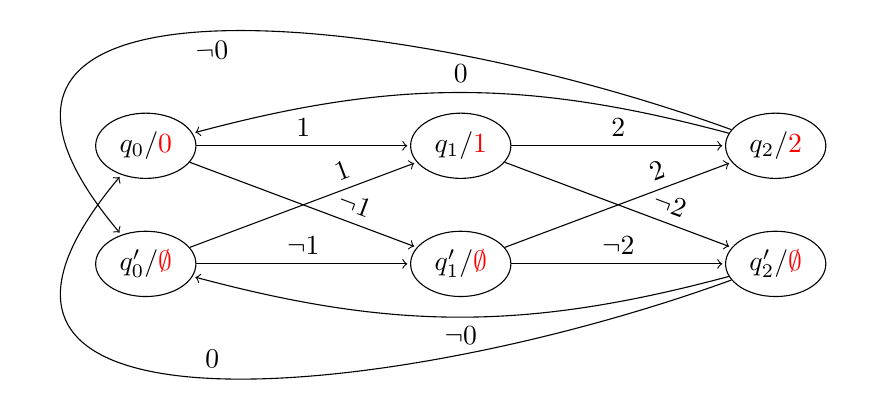
\begin{tikzpicture}[shorten >=1pt,node distance=1.5cm and 4cm,on grid,auto]
	\tikzset{state/.style={draw,ellipse,minimum size=0pt}};
		\clip (-1.5,1.5) rectangle (9, -3);
		\node[state] (q_0) {$q_0/{\color{red}0}$}; 
		\node[state] (q_1) [right=of q_0] {$q_1/{\color{red}1}$}; 
		\node[state] (q_2) [right=of q_1] {$q_2/{\color{red}2}$}; 
		\node[state] (q'_0) [below=of q_0] {$q'_0/{\color{red}\emptyset}$}; 
		\node[state] (q'_1) [below=of q_1] {$q'_1/{\color{red}\emptyset}$}; 
		\node[state] (q'_2) [below=of q_2] {$q'_2/{\color{red}\emptyset}$}; 
		\path[->] 
		(q_0)  edge node {$1$} (q_1)
		edge [sloped] node[pos=0.7] {$\lnot 1$} (q'_1)
		(q_1)  edge node {$2$} (q_2)
		edge [sloped] node [pos=0.7] {$\lnot 2$} (q'_2)
		(q_2)  edge [bend right=15, above] node {$0$} (q_0)
		edge [sloped, out=160, in=130, looseness=1.5, above] node  [below,pos=0.5] {$\lnot 0$} (q'_0)
		(q'_0) edge [sloped] node [pos=0.7] {$1$} (q_1)
		edge node {$\lnot 1$} (q'_1)
		(q'_1) edge [sloped] node [pos=0.7] {$2$} (q_2)
		edge node {$\lnot 2$} (q'_2)
		(q'_2) edge [sloped, out=200, in=230, looseness=1.5, below] node [above,pos=0.5] {$0$} (q_0)
		edge [bend left=15] node {$\lnot 0$} (q'_0)
		(q_2); 
	\end{tikzpicture}
	\caption{The transducer $\cT_i$ for Round Robin, initial state omitted. The input letters $\sigma$ and $\lnot\sigma$ mean all input letters from $2^\cP$ that, respectively, contain or do not contain $\sigma$. The labels are written in red on the states, singleton brackets omitted (e.g., ${\color{red} 1}$ means $\{1\}$).}
	\label{fig:RR}
\end{figure}

Technically, the initial state changes the behaviour of $\cT_i$ significantly (e.g. $\cT_0(\{0\}\{2\}\{1\})=\{0\}\emptyset\emptyset$ whereas $\cT_1(\{0\}\{2\}\{1\})=\emptyset\{2\}\emptyset$). Conceptually, however, changing the initial state does not alter the behaviour, as long as the requests are permuted accordingly. This is captured by round equivalence, as follows.

We argue that, if we allow reordering of the input letters, then the set of processes whose requests are granted in each round is independent of the start state. This is equivalent to saying $\cT_0 \equiv_k \cT_j$ for $j\in \{1,2\}$, which indeed holds: if $j=1$ then we permute all rounds of the form $\sigma_0 \sigma_1 \sigma_2$ to $\sigma_1 \sigma_2 \sigma_0$, and similarly if $j=2$ then we permute all rounds to $\sigma_2 \sigma_0 \sigma_1$. It is easy to see that the run of $\cT_i$ on the permuted input grants outputs that are permutations of the output of $\cT_0$ on the non-permuted input. 
\qed
\end{example}

\begin{example}[Round simulation is not symmetric]
\label{example:def-asymmetric}
Consider the $\sI/\sO$ transducers $\cT_1$ and $\cT_2$ over the alphabet $\sI=\{a,b\}$ and $\sO=\{0,1\}$, depicted in \autoref{fig:def-asymmetry}. 
\begin{figure}[ht]
	\centering
	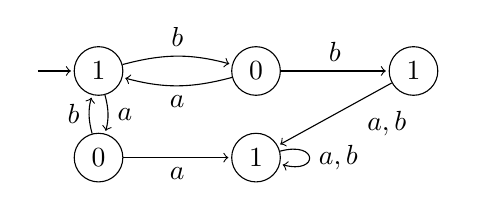
\begin{tikzpicture}[shorten >=1pt,node distance=1.1cm and 2cm,on grid,auto,initial text = {}]
	\clip (-0.9,0.55) rectangle (4.5, -1.5);
	    \tikzset{every state/.style={minimum size=0pt}}
		\node[state,initial] (q_0) {$1$}; 
		\node[state] (q_b) [right=of q_0] {$0$}; 
		\node[state] (q_a) [below=of q_0] {$0$}; 
		\node[state] (q_sink) [below=of q_b] {$1$}; 
		\node[state] (q_bb) [right=of q_b] {$1$}; 
		\path[->] 
		(q_0)  edge [bend left=15] node {$b$} (q_b)
		edge [bend left=15] node {$a$} (q_a)
		(q_b)  edge [bend left=15] node {$a$} (q_0)
		edge node {$b$} (q_bb)
		(q_bb) edge node[pos=0.3] {$a,b$} (q_sink)
		(q_a)  edge node[below] {$a$} (q_sink)
		edge [bend left=15] node {$b$} (q_0)
		(q_sink) edge [loop right] node {$a,b$} ();
	\end{tikzpicture}%
	\hspace{2cm}%
	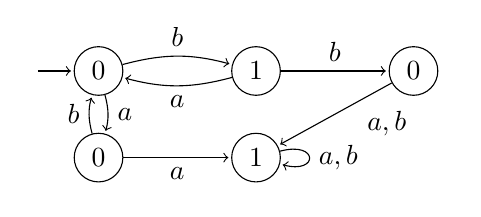
\begin{tikzpicture}[shorten >=1pt,node distance=1.1cm and 2cm,on grid,auto,initial text = {}]
	    \clip (-0.9,0.55) rectangle (4.5, -1.5);
	    \tikzset{every state/.style={minimum size=0pt}}
		\node[state,initial] (q_0) {$0$}; 
		\node[state] (q_b) [right=of q_0] {$1$}; 
		\node[state] (q_a) [below=of q_0] {$0$}; 
		\node[state] (q_sink) [below=of q_b] {$1$}; 
		\node[state] (q_bb) [right=of q_b] {$0$}; 
		\path[->] 
		(q_0)  edge [bend left=15] node {$b$} (q_b)
		edge [bend left=15] node {$a$} (q_a)
		(q_b)  edge [bend left=15] node {$a$} (q_0)
		edge node {$b$} (q_bb)
		(q_bb) edge node[pos=0.3] {$a,b$} (q_sink)
		(q_a)  edge node[below] {$a$} (q_sink)
		edge [bend left=15] node {$b$} (q_0)
		(q_sink) edge [loop right] node {$a,b$} ();
	\end{tikzpicture}%
	\caption{Transducers $\cT_1$ (left) and $\cT_2$ (right) illustrate the asymmetry in the definition of round equivalence (see \autoref{example:def-asymmetric}).}
	\label{fig:def-asymmetry}
\end{figure}
We claim that $\cT_1\prec_2 \cT_2$ but $\cT_2\not\prec_2 \cT_1$. Starting with the latter, observe that $\cT_2(ab)=00$, but $\cT_1(ab)=\cT_1(ba)=01$. Since $00\not\req[2]01$, we have $\cT_2\not\prec_2 \cT_1$. 

We turn to show that $\cT_1\prec_{2}\cT_2$.  Observe that for every input word of the form $x\in (ab+ba)^m$, we have $\cT_1(x)=(01)^m$, and $x\req[2] (ba)^m$. So in this case we have that $\cT_2((ba)^m)=(10)^m\req[2] (01)^m$. Next, for $x\in (ab+ba)^m\cdot bb\cdot w$ for some $w\in \sI^*$ we have $\cT_1(x)=(01)^m 01 1^{|w|}$ and $x\req[2] (ba)^m\cdot bb\cdot w$, for which $\cT_2((ba)^m\cdot bb\cdot w)=(01)^m 10 1^{|w|}\req[2]\cT_1(x)$.
The case where $x\in (ab+ba)^m\cdot aa\cdot w$ is handled similarly. We conclude that $\cT_1\prec_{2} \cT_2$.
\qed
\end{example}

Round simulation and round equivalence give rise to the following decision problems: 
\begin{itemize}
	\item In \emph{fixed round simulation} (resp. \emph{fixed round equivalence}) we are given transducers $\cT_1,\cT_2$, an \NFA for the language $\fL$, and $k>0$, and we need to decide whether $\cT_1\prec_{k,\fL} \cT_2$ (resp. whether $\cT_1\equiv_{k,\fL}\cT_2$).
	\item In \emph{existential round simulation} (resp. \emph{existential round equivalence}) we are given transducers $\cT_1,\cT_2$ and an \NFA for the language $\fL$, and we need to decide whether there exists $k>0$ such that $\cT_1\prec_{k,\fL} \cT_2$ (resp. $\cT_1\equiv_{k,\fL}\cT_2$). 
\end{itemize}
In the following we identify $\fL$ with an \NFA (or \DFA) for it, as we do not explicitly rely on its description.

We start by showing that deciding equivalence (both fixed and existential) is reducible, in polynomial time, to the respective simulation problem.
\begin{lemma}
	\label{lem:reduce_equiv_to_simulation}
Fixed (resp. existential) round equivalence is reducible in polynomial time to fixed (resp. existential) round simulation.
\end{lemma}
\begin{proof}
First, we can clearly reduce fixed round equivalence to fixed round simulation: given an algorithm that decides, given $\cT_1,\cT_2$, $\fL$ and $k>0$, whether $\cT_1\prec_{k,\fL} \cT_2$, we can decide whether $\cT_1\equiv_{k,\fL} \cT_2$ by using it twice to decide whether both $\cT_1\prec_{k,\fL} \cT_2$ and $\cT_1\prec_{k,\fL} \cT_2$ hold. 

A slightly more careful examination shows that the same approach can be taken to reduce existential round equivalence to existential round simulation, using the following observation: if $\cT_1\prec_{k,\fL} \cT_2$, then for every $m\in \bbN$ it holds that $\cT_1\prec_{mk,\fL}\cT_2$. Indeed, we can simply group every $m$ rounds of length $k$ and treat them as a single $mk$-round.

Now, given an algorithm that decides, given $\cT_1,\cT_2$ and $\fL$, whether there exists $k>0$ such that $\cT_1\prec_{k,\fL} \cT_2$, we can decide whether $\cT_1\equiv_{k,\fL} \cT_2$ by using the algorithm twice to decide whether there exists $k_1$ such that $\cT_1\prec_{k_1,\fL} \cT_2$ and $k_2$ such that $\cT_1\prec_{k_2,\fL} \cT_2$ hold. If there are no such $k_1,k_2$, then clearly $\cT_1 \not\equiv_{k,\fL} \cT_2$. However, if there are such $k_1,k_2$, then by the observation above we have $\cT_1\equiv_{k_1k_2,\fL}\cT_2$ (we can also take $\lcm(k_1,k_2)$ instead of $k_1k_2$).
\end{proof}
 
By \autoref{lem:reduce_equiv_to_simulation}, for the purpose of upper-bounds, we focus henceforth on round simulation.

\chapter{Conclusion and open questions}
\label{chap:conclusion}
\label{chap:discussion}
\label{chap:future}

This kind of chapter can include may different things (or only some of them):
\begin{itemize}
\item Discussion of results
\item Conclusions from the results or from the process in general
\item Open questions for future research, resulting from the research performed or from the results obtained
\end{itemize}

But not things like the bibliography or other back matter which is generated outside of this chapter.


\section{Some conclusion}

Here is what I conclude.

\section{Some open questions}

\paragraph{A question in brief.} In \autoref{chap:round_equivalence} we explored a certain subject, but what about this-or-that idea? Perhaps it is worth exploring. Can one produce interesting results?

\paragraph{A second question in brief.} A broader exposition of the question and indications of directions or ideas regarding its resolution.

In this work, we introduced round simulation and provided decision procedures and lower bounds (some with remaining gaps) for the related algorithmic problems.

Round simulation, and in particular its application to Round Symmetry, is only an instantiation of a more general framework of symmetry, by which we measure the stability of transducers under local changes to the input. In particular, we plan to extend this study to other definitions, such as \emph{window simulation}, where we use a sliding window of size $k$ instead of disjoint $k$-rounds, and \emph{Parikh round symmetry}, where the alphabet is of the form $2^{\cP}$, and we are allowed not only to permute the letters in each round, but also to shuffle the individual signals between letters in the round. 
In addition, the setting of infinite words is of interest, where one can define \emph{ultimate simulation}, requiring the simulation to only hold after a finite prefix. 
Finally, other types of transducers may require variants of simulation, such as probabilistic transducers, or streaming-string transducers~\cite{Alur2010}.

%
% Add any appendices here; they must come _before_ the bibliography
%
\appendix
%\noappendicestocpagenum
%\addappheadtotoc
\chapter{PSPACE Hardness}
\label{chap:apx}

\begin{lemma}
\label{lem:universalityofnfa}
Universality of \glspl{nfa} over alphabet $\Sigma=\{0,1\}$, where all states are accepting, and the degree of nondeterminism is at most $2$, is $\PSPACE$-complete.
\end{lemma}
\begin{proof}
In~\cite{kao2009nfas}, it is shown that universality of \glspl{nfa} remains $\PSPACE$-complete even for \glspl{nfa} over alphabet $\Sigma=\{0,1\}$ and all states accepting. Thus, we only need to show that this remains the case under the restriction that $|\delta(q,\sigma)|\le 2$ for every state $q$ and letter $\sigma$.

To see this, we start by observing that universality remains $\PSPACE$-complete for \glspl{nfa} over alphabet $\{0,1,\$\}$ with nondeterminism degree at most 2. Indeed, given an \gls{nfa} over $\{0,1\}$ with maximal nondeterminism degree $d>2$, we can replace each transition of the form\footnote{We can assume all transitions have degree exactly $d$ by adding redundant transitions} $\delta(q,\sigma)=\{q_1,\ldots, q_d\}$ with a binary tree of depth $\lceil \log d \rceil$, reading $\$$ on all transitions, which starts at $q$ and ends in $q_1,\ldots,q_d$. Thus, we introduce at most $d$ states for every transition. By marking these states as accepting, this reduction maintains universality, and requires a polynomial blowup.

Next, we observe that the reductions in~\cite[Lemma 2]{kao2009nfas} first transform an \gls{nfa} over alphabet size $k$ to an \gls{nfa} over alphabet size $k+1$ with all states accepting and with identical nondeterminism degree (indeed, the only added transitions are in fact deterministic), and then transforms an \gls{nfa} with all states accepting and alphabet size $4$ to an \gls{nfa} with all states accepting and alphabet size $2$, with an equal nondeterminism degree (essentially by encoding each of the 4 letters as two letters in $\{0,1\}$).

Since we start this chain of reductions with an \gls{nfa} of nondeterminism degree at most 2, we maintain this property throughout the proof.
\end{proof}

\section{Proof of~\cref{thm:equivalence_PSPACE-H}}
\label{apx:proof_equivalence_PSPACE-H}

We show a reduction from the universality problem for \glspl{nfa} over alphabet $\{0,1\}$ where all states are accepting and the degree of nondeterminism is at most 2, to round-equivalence with $k=2$ and with $\fL$ given as a \gls{dfa} of constant size. The former is shown to be $\PSPACE$-hard in~\cref{lem:universalityofnfa}.

Consider an \gls{nfa} $\cN=\tup{Q,\{0,1\},\delta,q_0,Q}$ where $|\delta(q,\sigma)|\le 2$ for every $q\in Q$ and $\sigma\in \{0,1\}$.
%Set $\Sigma=\{0,1\}$ and $\Lambda=(ab+cd)^*$, and let $A=\tup{Q, \Sigma, \delta,q_0,Q}$ be an \gls{nfa}. 
We construct two transducers $\cT_1$ and $\cT_2$ over input and output alphabets $\sI=\{a,b,c,d\}$ and $\sO=\{\top,\bot\}$ and $\fL\subseteq \sI^*$, such that $L(\cN)=\{0,1\}^*$ iff $\cT_1\equiv_{2,\fL}\cT_2$. 
%That is, iff for all $x\in \fL$ there exist $x'\req[2] x$ with $x'\in \fL$ and $x''\req[2] x$ that satisfy $\cT_1(x)\req[2] \cT_2(x')$ and $\cT_1(x'')\req[2] T_2(x)$.

Set $\fL=(ab+cd)^*$ (described as a 4-state \gls{dfa}). Intuitively, our reduction encodes $\{0,1\}$ into $\{a,b,c,d\}^2$ by setting $0$ to correspond to $ab$ and to $ba$, and $1$ to $cd$ and to $dc$. Then, $\cT_1$ keeps outputting $\top$ for all inputs in $\fL$, thus mimicking ``accepting'' every word in $\{0,1\}^*$. We then construct $\cT_2$ so that every nondeterministic transition of $\cN$ on e.g., $0$ is replaced by two deterministic branches on $ab$ and on $ba$. Hence, when we are allowed to permute $ab$ and $ba$ by round equivalence, we capture the nondeterminism of $\cN$. 

\begin{figure}[ht]
\begin{minipage}{.33\linewidth}
	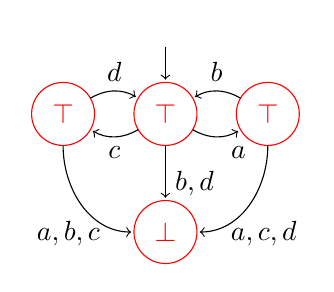
\begin{tikzpicture}[shorten >=1pt,node distance=1.5cm and 1.3cm,on grid,auto]
	    \tikzstyle{state}=[circle, inner sep=0mm, outer sep=0mm, minimum size=8mm, draw=black];
 	%   \clip (-2,0.9) rectangle (2.4, -1.3);
		\node[state] [initial text={\,}] (q_0) [red, initial above] {$\top$}; 
		\node[state] (q_1) [red, right=of q_0] {$\top$}; 
		\node[state] (q_2) [red, left=of q_0] {$\top$};
		\node[state] (q_3) [red, below=of q_0] {$\bot$};
		
		\path[->] 
		(q_0)
		 edge [bend right, swap, pos=0.6] node {$a$} (q_1)
		 edge [bend left] node {$c$} (q_2)
		 edge [pos=0.7] node {$b,d$} (q_3)
		(q_1) 
		 edge [bend right, swap] node {$b$} (q_0)
		 edge [out=-90, in=0] node[pos=0.8,yshift=0.2cm] {$a,c,d$} (q_3)
		(q_2)
	     edge [bend left] node {$d$} (q_0)
		 edge [out=-90, in=180, swap] node[pos=0.8,yshift=0.2cm] {$a,b,c$} (q_3);
	\end{tikzpicture}
 	\caption{The transducer $\cT_1$ in the proof of~\cref{thm:equivalence_PSPACE-H}.}
 	\label{fig:PSPACE_reduction_T1}
 \end{minipage}%
 \hfill%
 \begin{minipage}{.63\linewidth}
	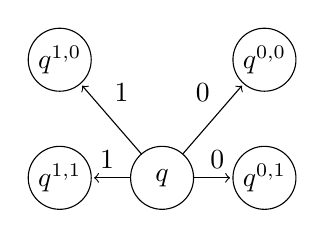
\begin{tikzpicture}[shorten >=1pt,node distance=1.5cm and 1.3cm,on grid,auto]
		\tikzstyle{state}=[circle, inner sep=0mm, outer sep=0mm, minimum size=8mm, draw=black];
		\node[state] (q_0) {$q$}; 
		\node[state] (q_1) [above right=of q_0] {$q^{0,0}$}; 
		\node[state] (q_2) [right=of q_0] {$q^{0,1}$}; 
		\node[state] (q_3) [above left=of q_0] {$q^{1,0}$}; 
		\node[state] (q_4) [left=of q_0] {$q^{1,1}$}; 
		
		\path[->] 
		(q_0)
		 edge node [pos=0.6] {$0$} (q_1)
		 edge node [pos=0.6] {$0$} (q_2)
		 edge node [pos=0.6, swap] {$1$} (q_3)
		 edge node [pos=0.6, swap] {$1$} (q_4);
	\end{tikzpicture}%
	\hspace{0.5cm}%
	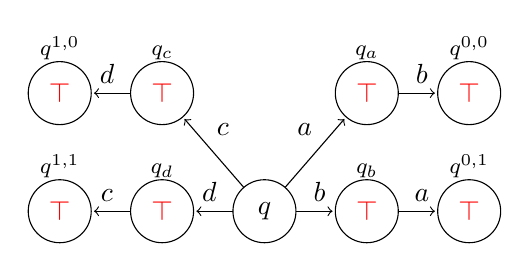
\begin{tikzpicture}[shorten >=1pt,node distance=1.5cm and 1.3cm,on grid,auto]
	    \tikzstyle{state}=[circle, inner sep=0mm, outer sep=0mm, minimum size=8mm, draw=black];
		\node[state] (q_0) {$q$}; 
		\node[state, label={[font=\footnotesize,label distance=-.1cm]above:$q_a$}] (q_1) [above right=of q_0] {$\color{red} \top$}; 
		\node[state, label={[font=\footnotesize,label distance=-.1cm]above:$q_b$}] (q_2) [right=of q_0] {$\color{red} \top$}; 
		\node[state, label={[font=\footnotesize,label distance=-.1cm]above:$q_c$}] (q_3) [above left=of q_0] {$\color{red} \top$}; 
		\node[state, label={[font=\footnotesize,label distance=-.1cm]above:$q_d$}] (q_4) [left=of q_0] {$\color{red} \top$}; 
		\node[state, label={[font=\footnotesize,label distance=-.1cm]above:$q^{0,0}$}] (q_1b)[right=of q_1] {$\color{red} \top$}; 
		\node[state, label={[font=\footnotesize,label distance=-.1cm]above:$q^{0,1}$}] (q_2b)[right=of q_2] {$\color{red} \top$}; 
		\node[state, label={[font=\footnotesize,label distance=-.1cm]above:$q^{1,0}$}] (q_3b)[left=of q_3] {$\color{red} \top$}; 
		\node[state, label={[font=\footnotesize,label distance=-.1cm]above:$q^{1,1}$}] (q_4b)[left=of q_4] {$\color{red} \top$}; 
		
		\path[->] 
		(q_0)
		 edge node [pos=0.6] {$a$} (q_1)
		 edge node [pos=0.6] {$b$} (q_2)
		 edge node [pos=0.6, swap] {$c$} (q_3)
		 edge node [pos=0.6, swap] {$d$} (q_4)
		(q_1) edge node [pos=0.6] {$b$} (q_1b)
		(q_2) edge node [pos=0.6] {$a$} (q_2b)
		(q_3) edge node [pos=0.6, swap] {$d$} (q_3b)
		(q_4) edge node [pos=0.6, swap] {$c$} (q_4b);
	\end{tikzpicture}
 	\caption{Every state and its 4 transitions in $\cN$ (left) turn into 8 transitions in $\cT_2$ (right). All transitions not drawn in the right figure lead to $q_\bot$, a sink state labelled $\color{red}\bot$.}
 	\label{fig:PSPACE_reduction_T2}
 \end{minipage}
\end{figure}

We now proceed to define the reduction formally. We construct $\cT_1$ independently of $\cN$, as depicted in~\cref{fig:PSPACE_reduction_T1}, containing 4 states. For every $x\in \fL$ we have $\cT_1(x)=\top^{|x|}$, and for every other $x\notin \fL$ we have $\cT_1(x)=\top^{m}\bot^{|x|-m}$ where $m$ is the length of the maximal prefix of $x$ in $(ab+cd)^*(a+c+\epsilon)$.

We proceed to construct $\cT_2$. 
%Recall that the nondeterminism degree of $\cN$ is $2$. Thus,
We can think of the outgoing transitions from every state $q$ as $\delta(q,0)=\{q^{0,0},q^{0,1}\}$ and $\delta(q,1)=\{q^{1,0},q^{1,1}\}$ (unless $\cN$ has no outgoing transitions on one of the letters, see below). We obtain $\cT_2$ from $\cN$ by introducing 4 new states $q_a,q_b,q_c,q_d$ for every state $q\in Q$, and setting the transitions and labels as depicted in~\cref{fig:PSPACE_reduction_T2}. In case $\cN$ does not have a transition on e.g., $0$ from $q$, then instead of going to $q_a$ or $q_b$, we proceed to a new state $q_\bot$ labelled $\bot$, which is a sink state. In addition, $q_\bot$ is reached upon any transition not yet defined.
Observe that for every $x\in \fL$ we have $\cT_2(x)=\top^{m}\bot^{|x|-m}$ for some $0\le m\le |x|$ (since $q_\bot$ is a sink).
% \begin{figure}
% \begin{minipage}{.30\linewidth}%[ht]
%  	%\centering
% 	\begin{tikzpicture}[shorten >=1pt,node distance=1cm and 1.5cm,initial distance=0.2cm,on grid,auto]
% 	\tikzstyle{smallnode}=[circle, inner sep=0mm, outer sep=0mm, minimum size=5mm, draw=black];
% 	%\clip (-5,2) rectangle (5, -4);
% 	\clip (-2,0.9) rectangle (2.4, -1.3);
% 		\node[smallnode, initial text={}] (q_0) [initial above] {$\color{red} \top$}; 
% 		\node[smallnode] (q_1) [right=of q_0] {$\color{red} \top$}; 
% 		\node[smallnode] (q_2) [left=of q_0] {$\color{red} \top$};
% 		\node[smallnode] (q_3) [below=of q_0] {$\color{red} \bot$};
		
% 		\path[->] 
% 		(q_0)
% 		 edge [bend right, swap, pos=0.6] node {$a$} (q_1)
% 		 edge [bend left] node {$c$} (q_2)
% 		 edge [pos=0.7] node {$b,d$} (q_3)
% 		(q_1) 
% 		 edge [bend right, swap] node {$b$} (q_0)
% 		 edge [out=-90, in=0] node[pos=0.8,yshift=0.2cm] {$a,c,d$} (q_3)
% 		(q_2)
% 	     edge [bend left] node {$d$} (q_0)
% 		 edge [out=-90, in=180, swap] node[pos=0.8,yshift=0.2cm] {$a,b,c$} (q_3);
% 	\end{tikzpicture}
%  	\caption{The transducer $\cT_1$ in the proof of~\cref{thm:equivalence_PSPACE-H}.}
%  	\label{fig:PSPACE_reduction_T1}
%  \end{minipage}%
%  \hfill%
%  %\hspace{2.0cm}%
%  \begin{minipage}{.65\linewidth}%[ht]
% 	%\centering
% 	\begin{tikzpicture}[shorten >=1pt,node distance=1cm and 1.2cm,on grid,auto]
% 		\tikzstyle{state}=[circle, inner sep=0mm, outer sep=0mm, minimum size=6mm, draw=black];
% 		%\clip (-2,1.5) rectangle (2,-0.4);
% 		\node[state] (q_0) {$q$}; 
% 		\node[state] (q_1) [above right=of q_0] {$q^{0,0}$}; 
% 		\node[state] (q_2) [right=of q_0] {$q^{0,1}$}; 
% 		\node[state] (q_3) [above left=of q_0] {$q^{1,0}$}; 
% 		\node[state] (q_4) [left=of q_0] {$q^{1,1}$}; 
		
% 		\path[->] 
% 		(q_0)
% 		 edge node [pos=0.6] {$0$} (q_1)
% 		 edge node [pos=0.6] {$0$} (q_2)
% 		 edge node [pos=0.6, swap] {$1$} (q_3)
% 		 edge node [pos=0.6, swap] {$1$} (q_4);
% 	\end{tikzpicture}%
% 	%\hspace{1cm}%
% 	\hspace{0.5cm}%
% 	\begin{tikzpicture}[shorten >=1pt,node distance=1cm and 1.2cm,on grid,auto]
% 	    \tikzstyle{state}=[circle, inner sep=0mm, outer sep=0mm, minimum size=6mm, draw=black];
% 	    %\clip (-3.5,2) rectangle (3.5,-0.4);
% 		\node[state] (q_0) {$q$}; 
% 		\node[state, label={[font=\footnotesize,label distance=-.1cm]above:$q_a$}] (q_1) [above right=of q_0] {$\color{red} \top$}; 
% 		\node[state, label={[font=\footnotesize,label distance=-.1cm]above:$q_b$}] (q_2) [right=of q_0] {$\color{red} \top$}; 
% 		\node[state, label={[font=\footnotesize,label distance=-.1cm]above:$q_c$}] (q_3) [above left=of q_0] {$\color{red} \top$}; 
% 		\node[state, label={[font=\footnotesize,label distance=-.1cm]above:$q_d$}] (q_4) [left=of q_0] {$\color{red} \top$}; 
% 		\node[state, label={[font=\footnotesize,label distance=-.1cm]above:$q^{0,0}$}] (q_1b)[right=of q_1] {$\color{red} \top$}; 
% 		\node[state, label={[font=\footnotesize,label distance=-.1cm]above:$q^{0,1}$}] (q_2b)[right=of q_2] {$\color{red} \top$}; 
% 		\node[state, label={[font=\footnotesize,label distance=-.1cm]above:$q^{1,0}$}] (q_3b)[left=of q_3] {$\color{red} \top$}; 
% 		\node[state, label={[font=\footnotesize,label distance=-.1cm]above:$q^{1,1}$}] (q_4b)[left=of q_4] {$\color{red} \top$}; 
		
% 		\path[->] 
% 		(q_0)
% 		 edge node [pos=0.6] {$a$} (q_1)
% 		 edge node [pos=0.6] {$b$} (q_2)
% 		 edge node [pos=0.6, swap] {$c$} (q_3)
% 		 edge node [pos=0.6, swap] {$d$} (q_4)
% 		(q_1) edge node [pos=0.6] {$b$} (q_1b)
% 		(q_2) edge node [pos=0.6] {$a$} (q_2b)
% 		(q_3) edge node [pos=0.6, swap] {$d$} (q_3b)
% 		(q_4) edge node [pos=0.6, swap] {$c$} (q_4b);
% 	\end{tikzpicture}
%  	\caption{Every state and its 4 transitions in $\cN$ (left) turn into 8 transitions in $\cT_2$ (right). All transitions not drawn in the right figure lead to $q_\bot$, a sink state labelled $\color{red}\bot$.}
%  	\label{fig:PSPACE_reduction_T2}
%  \end{minipage}
% \end{figure}
%Assume $\Sigma^* = L(A)$, then all words have a path. Let $x\in\Lambda$. It is straightforward to see that $T_1(x)=\mathbf{o}_1^{|x|}$. Moreover, $T_2(x')=\mathbf{o}_1^{|x|}$, where $x'$ is obtained as follows: Replace every appearance of $ab$ with $0$ and of $cd$ with $1$, and call the resulting word $\hat{x}$. This word has a generating path in $A$, denoted by $s_1\rightarrow s_2\rightarrow\cdots\rightarrow s_k$. Now, every path in $A$ has a matching path in $T_1$ (in a one-to-one manner).

We now claim that $L(\cN)=\{0,1\}^*$ iff $\cT_1\equiv_{2,\fL}\cT_2$.
For the first direction, assume $L(\cN)=\{0,1\}^*$. Observe that $\cT_2\prec_{2,\fL}\cT_1$ independently: for every $x\in (ab+cd)^*$, denote $\cT_2(x)=\top^{m}\bot^{|x|-m}$, then we can construct $x'\req[2]x$ such that $\cT_1(x')=\top^{m}\bot^{|x|-m}$ by leaving $x$ unchanged $m$ steps, and then permuting the letters such that the run of $\cT_1$ moves to the sink labelled $\bot$ (indeed, observe that $m$ must be even by the construction of $\cT_2$, and hence $\cT_1$ can permute e.g., $ab$ to $ba$ in order to start outputting $\bot$ on an even step).

Next, we show that $\cT_1\prec_{2,\fL}\cT_2$. Consider $x\in (ab+cd)^*$, so that $\cT_1(x)=\top^{|x|}$, and let $w\in \{0,1\}^*$ be the word obtained from $x$ by identifying $ab$ with $0$ and $cd$ with $1$. Since $L(\cN)=\{0,1\}^*$, there exists a run (and hence an accepting run) of $\cN$ on $w$, denoted $s_0,s_1,\ldots,s_n$. We now obtain $x''\req[2]x$ by identifying each letter $0$ in $x$ with either $ab$ or $ba$, and each letter $1$ with $cd$ or $dc$, such that the run of $\cT_2$ on $x''$ simulates the run of $\cN$ on $w$. Thus, $\cT_2(x'')=\top^{|x''|}$, and $\cT_2(x'')\req[2]\cT_1(x)$, so we are done.

Conversely, if $\cT_1\equiv_{2,\fL}\cT_2$, then in particular $\cT_1\prec_{2,\fL}\cT_2$. We claim that $L(\cN)=\{0,1\}^*$. Consider $w\in \{0,1\}^*$. Dually to the above, we obtain from $w$ a word $x\in (ab+cd)^*$ by identifying $0$ with $ab$ and $1$ with $cd$, so that $\cT_1(x)=\top^{|x|}$. 
Since $\cT_1\prec_{2,\fL}\cT_2$, there exists $x'\req[2]x$ such that $\cT_2(x')=\top^{|x|}$. Observe that $x'$ must be obtained from $x$ by (possibly) changing each $ab$ to $ba$ and each $cd$ to $dc$. In particular, the run of $\cT_2$ on $x'$ induces a run of $\cN$ on $w$ by identifying both $ab$ and $ba$ as 0 and both $cd$ and $dc$ as 1. This gives $w\in L(\cN)$, so $L(\cN)=\{0,1\}^*$, which concludes the proof. \qed

\section{Proof of~\cref{thm:existential_equivalence_PSPACE-H}}
\label{apx:proof_existential_PSPACE-H}

In order to show that existential round equivalence is $\PSPACE$-hard, we build upon the reduction in the proof of Theorem~\ref{thm:equivalence_PSPACE-H}: we again show a reduction from the universality problem for \glspl{nfa} over alphabet $\{0,1\}$ where all states are accepting and the degree of nondeterminism is at most 2 (cf.~\cref{lem:universalityofnfa}).

Consider an \gls{nfa} $\cN=\tup{Q,\{0,1\},\delta,q_0,Q}$ where $|\delta(q,\sigma)|\le 2$ for every $q\in Q$ and $\sigma\in \{0,1\}$.
We construct two transducers $\cT_1$ and $\cT_2$ over input and output alphabets $\sI=\{a,b,c,d,\#\}$ and $\sO=\{\top,\bot\}$ and $\fL\subseteq \sI^*$, such that $L(\cN)=\{0,1\}^*$ iff $\cT_1\equiv_{2,\fL}\cT_2$. 

Intuitively, the idea is to use a similar encoding of $\{0,1\}$ in $\{a,b,c,d\}$ whereby $0$ corresponds to either $ab$ or $ba$ and $1$ to $cd$ or $dc$. Now, however, since $k$ is not fixed to $2$, we also allow arbitrary padding with sequences of $\#\#$.

Set $\fL=(ab+cd+\#\#)^*$ (given as a 5 state \gls{dfa}). We construct $\cT_1$ and $\cT_2$ similarly to the proof of~\cref{thm:equivalence_PSPACE-H}, by adding self-cycles of length 2 upon reading $\#\#$, from every state except the sink $q_\bot$. See~\cref{fig:existential_PSPACE_reduction_T1,fig:existential_PSPACE_reduction_T2} for an illustration.

\begin{figure}[ht]
	\centering
	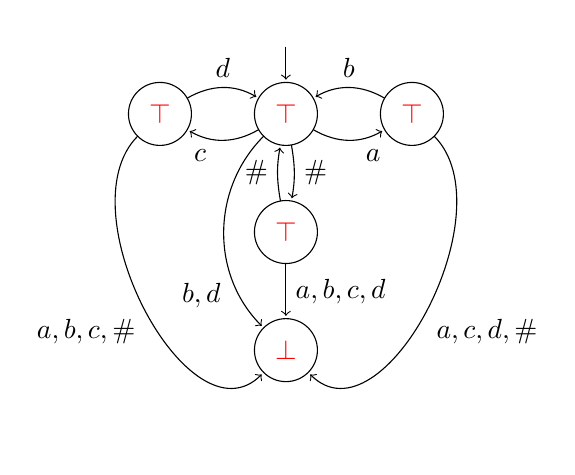
\begin{tikzpicture}[shorten >=1pt,node distance=1.5cm and 1.6cm,on grid,auto]
	\tikzstyle{smallnode}=[circle, inner sep=0mm, outer sep=0mm, minimum size=8mm, draw=black];
		\node[smallnode] [initial text={}] (q_0) [initial above] {$\color{red} \top$}; 
		\node[smallnode] (q_1) [right=of q_0] {$\color{red} \top$}; 
		\node[smallnode] (q_2) [left=of q_0] {$\color{red} \top$};
		\node[smallnode] (q_3) [below=of q_0] {$\color{red} \top$};
		\node[smallnode] (q_4) [below=of q_3] {$\color{red} \bot$};
		
		\path[->] 
		(q_0)
		 edge [bend right, swap, pos=0.6] node {$a$} (q_1)
		 edge [bend left, pos=0.6] node {$c$} (q_2)
		 edge [bend left=10] node {$\#$} (q_3)
		 edge [out=-135, in=135, swap, pos=0.7] node {$b,d$} (q_4)
		(q_1) 
		 edge [bend right, swap] node {$b$} (q_0)
		 edge [out=-45, in=-45] node {$a,c,d,\#$} (q_4)
		(q_2)
	     edge [bend left] node {$d$} (q_0)
		 edge [out=-135, in=-135, swap] node {$a,b,c,\#$} (q_4)
		(q_3)
		 edge [bend left=10] node {$\#$} (q_0)
		 edge [] node {$a,b,c,d$} (q_4);
		 
	\end{tikzpicture}
	\caption{The transducer $\cT_1$ in  the proof of~\cref{thm:existential_equivalence_PSPACE-H}.}
	\label{fig:existential_PSPACE_reduction_T1}
\end{figure}

\begin{figure}[ht]
	\centering
	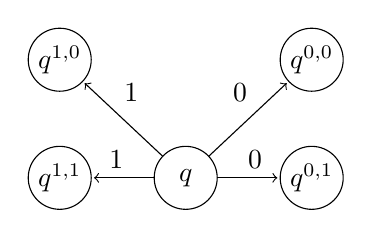
\begin{tikzpicture}[shorten >=1pt,node distance=1.5cm and 1.6cm,on grid,auto]
		\tikzstyle{state}=[circle, inner sep=.5mm, outer sep=0mm, minimum size=8mm, draw=black];
		\node[state] (q_0) {$q$}; 
		\node[state] (q_1) [above right=of q_0] {$q^{0,0}$}; 
		\node[state] (q_2) [right=of q_0] {$q^{0,1}$}; 
		\node[state] (q_3) [above left=of q_0] {$q^{1,0}$}; 
		\node[state] (q_4) [left=of q_0] {$q^{1,1}$}; 
		
		\path[->] 
		(q_0)
		 edge node [pos=0.6] {$0$} (q_1)
		 edge node [pos=0.6] {$0$} (q_2)
		 edge node [pos=0.6,swap] {$1$} (q_3)
		 edge node [pos=0.6,swap] {$1$} (q_4);
	\end{tikzpicture}%
	\hspace{2cm}%
	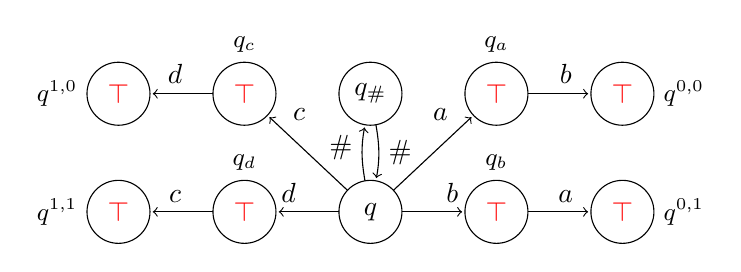
\begin{tikzpicture}[shorten >=1pt,node distance=1.5cm and 1.6cm,on grid,auto]
	    \tikzstyle{state}=[circle, inner sep=.5mm, outer sep=0mm, minimum size=8mm, draw=black];
		\node[state] (q_0) {$q$}; 
		\node[state] (q') [above=of q_0] {$q_\#$}; 
		\node[state, label={[font=\small]above:$q_a$}] (q_1) [above right=of q_0] {$\color{red} \top$}; 
		\node[state, label={[font=\small]above:$q_b$}] (q_2) [right=of q_0] {$\color{red} \top$}; 
		\node[state, label={[font=\small]above:$q_c$}] (q_3) [above left=of q_0] {$\color{red} \top$}; 
		\node[state, label={[font=\small]above:$q_d$}] (q_4) [left=of q_0] {$\color{red} \top$}; 
		\node[state, label={[font=\small]right:$q^{0,0}$}] (q_1b)[right=of q_1] {$\color{red} \top$}; 
		\node[state, label={[font=\small]right:$q^{0,1}$}] (q_2b)[right=of q_2] {$\color{red} \top$}; 
		\node[state, label={[font=\small]left:$q^{1,0}$}] (q_3b)[left=of q_3] {$\color{red} \top$}; 
		\node[state, label={[font=\small]left:$q^{1,1}$}] (q_4b)[left=of q_4] {$\color{red} \top$}; 
		
		\path[->] 
		(q_0)
		 edge node [pos=0.8] {$a$} (q_1)
		 edge node [pos=0.8] {$b$} (q_2)
		 edge node [pos=0.8, swap] {$c$} (q_3)
		 edge node [pos=0.8, swap] {$d$} (q_4)
		 edge [bend left=10, pos=0.6] node {$\#$} (q')
		(q_1) edge node [pos=0.6] {$b$} (q_1b)
		(q_2) edge node [pos=0.6] {$a$} (q_2b)
		(q_3) edge node [pos=0.6, swap] {$d$} (q_3b)
		(q_4) edge node [pos=0.6, swap] {$c$} (q_4b)
		(q') edge [bend left=10, pos=0.5] node {$\#$} (q_0);
	\end{tikzpicture}
	\caption{Every state and its 4 transitions in $\cN$ (left) turn into 10 transitions in $\cT_2$ (right). All transitions not drawn in the right figure lead to $q_\bot$, a sink state labelled $\color{red}\bot$.}
	\label{fig:existential_PSPACE_reduction_T2}
\end{figure}

We claim that $L(\cN)=\{0,1\}^*$ iff there exists $k>0$ such that $\cT_1\equiv_{k,\fL}\cT_2$.
For the first direction, assume $L(\cN)=\{0,1\}^*$, then we can show that $\cT_1\equiv_{2,\fL}\cT_2$ by following the proof of~\cref{thm:equivalence_PSPACE-H} line for line, with the addition that blocks of the form $\#\#$ leave the state of both $\cT_1$ and $\cT_2$ unchanged.

For the converse direction, assume $\cT_1\equiv_{k,\fL}\cT_2$, and in fact we only assume $\cT_1\prec_{k,\fL}\cT_2$ for some $k>0$. We further assume w.l.o.g.\! that $k$ is even, otherwise we can just take $2k$ (since we also have $\cT_1\prec_{2k,\fL}\cT_2$).

Consider $w\in \{0,1\}^*$. We obtain from $w$ a word $x\in (ab+cd+\#\#)^*$ by identifying $0$ with $ab\#^{k-2}$ and $1$ with $cd\#^{k-2}$. Observe that $\cT_1(x)=\top^{|x|}$, and that $x$ is indeed a $k$-round word in $\fL$, with each round being either $ab\#^{k-2}$ or $cd\#^{k-2}$. 

Since $\cT_1\prec_{k,\fL}\cT_2$, there exists $x'\req[k]x$ such that $\cT_2(x')=\top^{|x|}$. Observe that $x'$ must be obtained from $x$ by (possibly) changing each $ab$ to $ba$ and each $cd$ to $dc$, and by shifting the location of this pair within the $\#$ symbols. Indeed, otherwise the run of $\cT_2$ on $x'$ ends in $q_{\bot}$.
In particular, the run of $\cT_2$ on $x'$ induces a run of $\cN$ on $w$ by identifying both $ab$ and $ba$ as 0 and both $cd$ and $dc$ as 1. Thus, $w\in L(\cN)$, so $L(\cN)=\{0,1\}^*$, and the proof is concluded. \qed

% \begin{section}
% This a former try of proving existential. Either Appendix or drop.

% \begin{hypothesis}
% Let $A,B$ be two \glspl{nfa} over $\Sigma$. There exists a bound $M=M(A,B)$ that satisfies the following: let $x\in \Sigma^\star$ and $x'\equiv x$ a permutation thereof. Denote $q'\in\delta_1(q,x)$ and $s'\in\delta_2(s,x')$, then there exists such an $x$ with $|x|<M$.
% \end{hypothesis}

% To understand how this theorem can help our cause, recall that the algorithm for checking $k$-simulation in rounds was based on a construction of a \gls{dfa} $A_1^k$ and an \gls{nfa} $A_2^k$ so that, if we fix $T_1$ and $T_2$ and gradually increase $k$, we will have a sequence of automata with identical states, wherein only the transitions and the alphabet change.

% If we succeed to show that for some $k_1$ and $k_2$ the two pairs of automata are identical in transitions, then by help of the theorem we can bound the difference $k_2-k_1$ and hopefully get a deterministic analysis of the values of $k$ which would work, i.e. we would solve the problem of bounding $k$.

% \end{section}


% Back Matter
% ------------

% The following command will typeset the bibliography,
% then typeset the Hebrew part of the thesis:
% - Cover page
% - Title page
% - Acknowledgements page
%  (NO table of contents or list of figures in Hebrew)
% - (Extended) abstract (1000-2000 words)
%
% based on information you've provided in the thesis-fields file
% (including the relative paths to your bib files). The Hebrew
% content will be typeset in _reverse_page_order_, i.e. first
% in the file will be the last page of the abstract, and the
% Hebrew cover page will be the last page of the file.
%
\makebackmatter

% The resulting PDF can be printed and taken straight to binding,
% i.e. you do not need to flip any pages anywhere. Of course,
% mind the LaTeX error and warning messages, overfull hboxes etc.

\end{document}

